\chapter{Finite-Word Relations and Automatic Structures}
\label{ch:preliminaries-automatic-structures}

\begin{chapterpresentation}
	\begin{abstract}
		This preliminary chapter surveys the literature on
		the notion of \emph{rationality} for finite word relations and
		"automatic structures".

		We start by reviewing competing definitions of rationality for $k$-ary
		relations of finite words ($k \geq 2$).
		We survey the corresponding hierarchy, which is mainly shaped
		by the expressive power of "multitape automata". We also
		briefly mention other models such as transducers to emphasize their
		relationship with our hierarchy.
		"Automatic relations" naturally emerge as one of the most expressive class of
		relations having desirable closure properties and
		for which most ``basic'' problems are decidable.

		After a brief logical interlude mostly dedicated to logical characterizations of 
		"automatic relations", we move on to "automatic structures", which
		are infinite "relational structures" that can be finitely described using
		"automatic relations". As a result, the first-order theory of such structures
		is decidable, explaining why "automatic structures" play a central role
		when looking for algorithms dealing with infinite "structures".
		Unfortunately, other decision problems, such as the "isomorphism problem",
		are undecidable, but become decidable when restricted to a specific
		subclass of structures. We hence conclude this chapter by
		discussing the computability status of natural decision problems
		on "automatic structures".
	\end{abstract}
	\par\bigskip\bigskip
	\begin{acknowledgements}
		Parts of \Cref{sec:preliminaries-automatic-structures-relations}
		come from \cite[\S~1]{Morvan2025Algebras} and \cite[\S~B]{Morvan2025Algebras}.
	\end{acknowledgements}
	\clearpagepresentation
	\chaptertocstandalone
\end{chapterpresentation}

% \epigraph{On sait ce qu'est une vache, mais on ne sait pas ce qu'est « pas une vache ».}{Igor Walukiewicz}
% On the subject of ``asynchronous automata''.

\section{The Landscape of Rationality for Relations over Finite Words}
\label{sec:preliminaries-automatic-structures-relations}

\subsection{Regularity is Key...}

The class of "regular languages" is remarkably stable, and can either be characterized as the 
languages recognized by either:
\begin{itemize}
	\item deterministic or non-deterministic finite state automata,\\
		\null\hspace{1.0pc}see "eg" \cite[Proposition~1.2.3, p.~7]{Pin2021FiniteAutomata};
	\item two-way finite state automata by Shepherdson-Rabin-Scott theorem\\
		\null\hspace{1.0pc}\cite[Theorem~2, p.~198]{Shepherdson1959ReductionTwoWay}
		\cite[Theorem~15, p.~123]{RabinScott1959FiniteAutomata};
	\item rational expressions by Kleene's theorem,\\
		\null\hspace{1.0pc}see "eg" \cite[Theorem~1.5.11, p.~34]{Pin2021FiniteAutomata};
	\item monadic second-order logic by Trakhtenbrot-Büchi-Elgot theorem,\\
		\null\hspace{1.0pc}see "eg" \cite[Theorem~2.2, p.~32]{Bojanczyk2020MSO}; or
	\item finite monoids, see "eg" \cite[\S~1.4.2, p.~19]{Pin2021FiniteAutomata}.
\end{itemize}
Moreover, all transformations between these representations are effective---although some
models can be strictly more succinct.

\begin{figure*}
	\centering
	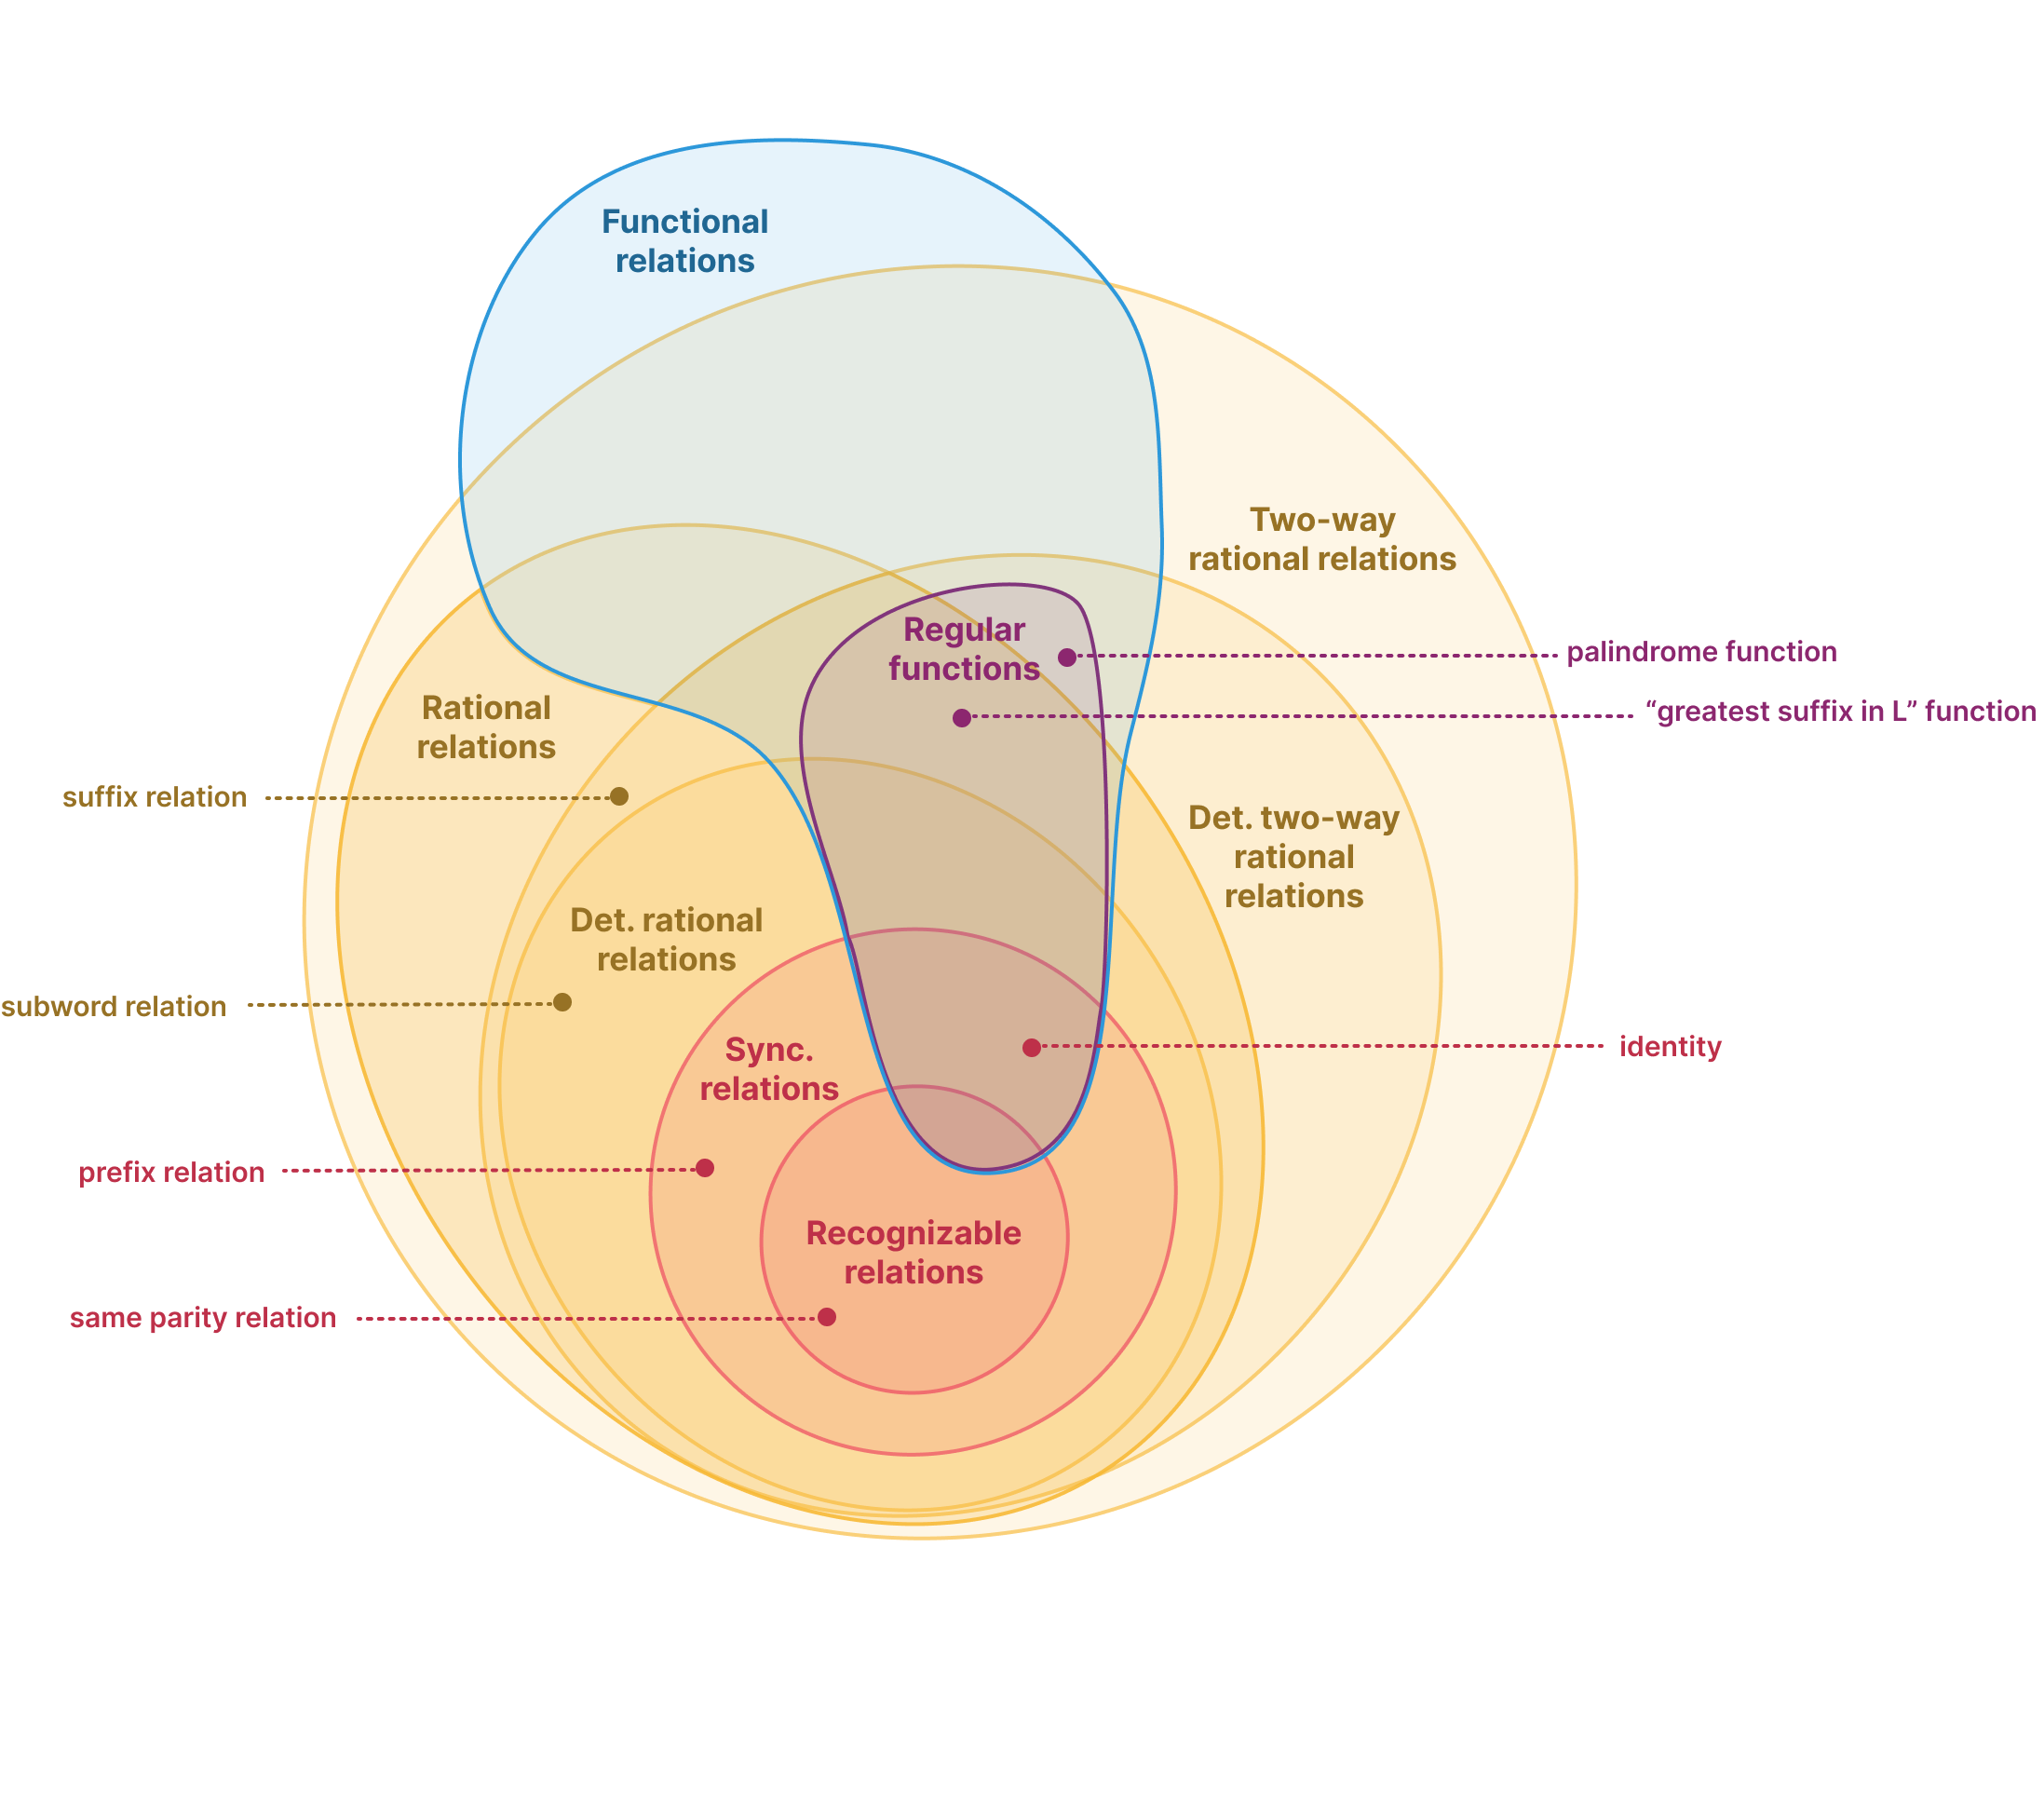
\includegraphics[width=\linewidth]{fig/landscape-rationality-relations.png}
	\caption{
		\AP\label{fig:landscape-rationality-relations}
		The ``landscape of rationality'' for binary relations.
		Dashed regions are empty.
		TODO:UPDATE: SUFFIX RELATION IS Deterministic TWO-WAY AND RATIONAL.
	}
\end{figure*}
These equivalences explain why the terms \emph{recognizable language}---meaning implicitly
``recognizable by a finite-state automaton'' or ``recognizable by a finite monoid''---and
\emph{rational language}---meaning ``described by a rational expression''---are used 
interchangeably. In fact, in this thesis as well as in most of the literature,
we will use the generic term "regular language".
However, in more complex settings, for instance subsets of non-free monoids,%
\footnote{Recall that a language is nothing else but a subset of a free
(usually finitely-generated) monoid.}
the equivalence between these classes no longer holds. \cite{Pin2021StackExchange}

The landscape of rationality for $k$-ary relations of finite words ($k \geq 2$) is far more complex than for languages,\footnote{Which can be seen as unary relations of finite words.} as depicted in \Cref{fig:landscape-rationality-relations}. We will briefly present these classes,
although this thesis will only deal with the two most restrictive ones, namely
"recognizable@@rel" and "automatic relations".%
\footnote{It should be noted that the names
of these classes were often coined independently of one another---sometimes defying common sense.
For instance, "automatic relations" are named this way because they correspond to
the relations recognized by some model of automata...
not unlike most of the classes in \Cref{fig:landscape-rationality-relations}.
They are also sometimes named ``regular relations'', which have nothing to do
with "regular functions" and do \emph{not} correspond to the intersection of "regular functions"
with "functional relations", as one would reasonably expect.}
We fix two alphabets $\Gamma$ and $\Sigma$. In the rest of this section, we focus
on relations $\+R \subseteq \Gamma^* \times \Sigma^*$, "aka" transductions.

\paragraph*{Goal of this section.}
When I learned about these classes, I was somewhat confused between the different models: surprisingly, the literature on transductions seems somewhat orthogonal to the one on relation.%
\footnote{For instance \cite{Choffrut2006Survey} mentions todo, but not todo. On the other hand todo.}
The goal of this section is to provide a non-exhaustive overview of these classes of relations/transductions, explain how they relate to one another, and give pointers to suitable references.
We acknowledge \cite{Choffrut2006Survey}, which proved particularly useful to find the
appropriate references. Of course, the aim of this section is not to be exhaustive,
which would be a daunting task,%
\footnote{Sakarovitch's book \cite{Sakarovitch2009Elements}
dedicates its second part to ``Rationality in relations'', which spans over more than two hundred pages---one can only imagine how extensive this part could have been if the book was not
dedicated to presenting \emph{elements} of automata theory but the full theory itself!}
but rather to present a quick overview of the most common classes of relations
studied in the literature.
todo:most can be skipped.

\paragraph*{Relations "vs" transductions.}
Often, in the literature, when the terminology ``transduction'' is used,
these relations are thought as functions from $\Gamma^*$ to $\pset{\Sigma^*}$---sometimes
assuming that the input is a singleton, sometimes not---,
and in this case $\Gamma$ (resp. $\Sigma$) plays the role of an ``input alphabet''
(resp. ``output alphabet''). A transducer reads a letter from the input alphabet,
and \emph{produces} a letter from the output alphabet: inherently, transducers are seen
as a machine that \emph{produces} an ouput, or rather that \emph{tranduces} an input into an output, or multiple outputs.

On the other hand, when the terminology ``relation'' is used,
we often take $\Gamma = \Sigma$.\footnote{For instance this is somewhat important when
dealing with logic or defining automatic structure
\Cref{sec:preliminaries-automatic-structures-automatic-structures,sec:preliminaries-automatic-structures-logic}.}
Multitape automata are seen as machine that read
tuples of words, and either accept or reject them: it is a decision model.
The question of $\Gamma =^? \Sigma$ makes little difference since we can often
see a relation $\+R \subseteq \Gamma^* \times \Sigma^*$ as a subset of
$(\Gamma\sqcup \Sigma)^* \times (\Gamma\sqcup \Sigma)^*$
while preserving the notion of ``rationality'' at hand.
Moreover, we will see that some classes can be equally defined
by using multitape automata or transducers todo:addref.

Note also that most notions defined by multitape automata
can be trivially extended to $k$-ary relations ($k \geq 3$):
we simply work here with binary relations for the sake of simplicity---we will sometimes give more general definition for higher arity when the generalization is not trivial.
On the other hand, transducers intrinsically recognize functions $\Gamma^* \to \pset{\Sigma^*}$,
"ie" binary relations.

Given two classes of finite-word relations $\+C$ and $\+D$ "st" $\+C \supseteq \+D$,
we will often want to know if this inclusion is \emph{effective}:
\decisionproblem{
	""$\+D$-membership problem for $\+C$-relations""
}{
	A $\+C$-relation $\+R$.
}{
	Does $\+R \in \+D$?
}
This problem is also called the \reintro{$\+C$/$\+D$-membership problem}.

A natural extension of this problem is the so-called separability problem,
which has received lots of attention in todo:addref.
\decisionproblem{
	""$\+D$-separability problem for $\+C$-relations""
}{
	Two $\+C$-relations $\+R$ and $\+R'$.
}{
	Is there a $\+D$-relation "st" $\+R \subseteq \+S$ and $\+R' \cap \+S = \emptyset$?
}
In this case, we say that $\+S$ ""separates@@rel"" $\+R$ from $\+R'$.
Note that when $\+D$ is closed under complement, $\+R$ and $\+R'$ play a symmetric role in this problem. Moreover, if $\+D$ is \emph{effectively} closed under complement,
then "membership@@problemrel" reduces to "separability@@problemrel" 
since $\+R in \+D$ if, and only if, $\+R$ and its complement are "separable@@rel" by
a $\+D$-relation.


\subsection{Recognizable Relations}

A relation $\+R \subseteq \Gamma^* \times \Sigma^*$ is \AP""recognizable@@rel""
if there exists a "finite monoid" $\?M$ together with a "monoid morphism"
\[
	f\colon \Gamma^* \times \Sigma^* \to \?M,
\]
as well as a subset $\Acc \subseteq M$ "st"
$\+R = f^{-1}[\Acc]$. We denote by \AP$\intro*\REC$ the class of "recognizable relations".%
\footnote{todo: Again, insert some set-theoretic bullshit.}

For instance the \AP""same parity relation""
\[
	{\intro*\sameParity} \defeq 
	\{
		\tup{u,v} \in \Gamma^* \times \Sigma^* \mid
		|u| = |v| \mod{2}
	\}
\]
is "recognizable@@rel". Indeed, letting $f\colon  \Gamma^* \times \Sigma^* \to \ZnZ{2}$,
then $\sameParity$ can be written as $f^{-1}[\{\bar 0\}]$.

These relations admit a remarkably simple characterization.\AP
\begin{proposition}[{""Mezei theorem"", see "eg" \cite[Corollary~II.2.20, p.~254]{Sakarovitch2009Elements}}]
	\!\footnote{\cite[\S~2, ``Notes \& references'']{Sakarovitch2009Elements} mentions
	that this proposition is ``unanimously ascribed to G. Mezei (unpublished)''.}
	\label{prop:Mezei-theorem}
	A relation $\+R$ is "recognizable@@rel" "iff" there exists $n\in\N$,
	"regular languages" $\tup{K_i}_{i\in \lBrack 1,n\rBrack}$ over $\Gamma$
	and "regular languages" $\tup{L_i}_{i\in \lBrack 1,n\rBrack}$ over $\Sigma$
	"st"
	\[
		\+R = \bigcup_{i=1}^n K_i \times L_i.
	\]
\end{proposition}

In other words, "recognizable relations" are exactly the finite unions of
"Cartesian products" of "regular languages".
For instance, \[{\sameParity} =
(\Gamma\Gamma)^* \times (\Sigma\Sigma)^*
\cup \Gamma(\Gamma\Gamma)^* \times \Sigma(\Sigma\Sigma)^*.\]
We provide a slightly more general statement of "Mezei theorem".

\begin{proposition}
	\label{prop:Mezei-theorem-generalization}
	Let $\B{V}$ be a "pseudovariety of finite monoids"
	and $\+V$ be the corresponding "pseudovariety of regular languages".
	Let $\+R \subseteq \Gamma^* \times \Sigma^*$ be a relation.
	The following are equivalent:
	\begin{enumerate}
		\item there exists a "finite monoid" $\?M \in \B{V}$, a "monoid morphism"
		$f\colon \Gamma^* \times \Sigma^* \to \?M$ and $\Acc \subseteq \?M$
		"st" $\+R = f^{-1}[\Acc]$;
		\item there exists $n \in \N$
		and $K_1,\hdots,K_n \in \+V_{\Gamma}$ and $L_1,\hdots,L_n \in \+V_{\Sigma}$
		"st" $\mathcal{R} = \bigcup_{i=1}^n K_i \times L_i$,
	\end{enumerate}
	in which case we say that $\+R$ is \AP""$\+V$-recognizable@@rel"".
\end{proposition}

When $\B{V}$ is the "pseudovariety@@reglang" of all "regular languages",
we get back \Cref{prop:Mezei-theorem}.

\begin{proof}
	\proofcase{From monoids to products.}
	Assume that $\+R$ is "recognizable@@rel". 
	Then by definition
	\[
		\+R = \bigcup_{z \in \Acc} f^{-1}[z].
	\]
	Observe then that $f(u,v) = f(\tup{u,\varepsilon}\cdot\tup{\varepsilon,v})
	= f(u,\varepsilon)\cdot f(\varepsilon,v)$ for all $u,v \in \Gamma^* \times \Sigma^*$, and hence:
	\[
		\+R = \bigcup_{\substack{x,y \in M\\ \text{"st" } x\cdot y \in \Acc}}
		\underbrace{\{u \in \Gamma^* \mid f(u, \varepsilon) = x\}}_{\defeq \;K_x}
		\times \underbrace{\{v \in \Sigma^* \mid f(\varepsilon, v) = y\}}_{\defeq \;L_y}.
	\]
	Since $M$ is finite, the union is finite, and moreover, each $K_x$ and $L_y$ is
	recognized by $M \in \B{V}$, and hence belong to $\+V$.

	\proofcase{From products to monoids.} If $\mathcal{R} = \bigcup_{i=1}^n K_i \times L_i$ 
		where all languages belong to $\+V$, then let $M_i,N_i \in \B{V}$
		be their "syntactic monoids", $g_i,h_i$ be their
		"syntactic morphism", and $\Acc_i,\Bcc_i$ be their accepting sets.
		Consider the monoid morphism
		\begin{center}
		\begin{tabular}{ccc}
			$\Gamma^* \times \Sigma^*$ & $\to$ & $\prod_{i}(M_i \times N_i)$ \\
			$\tup{u,v}$ & $\mapsto$ & $\tup{g_i(u), h_i(v)}_{i}$.
		\end{tabular}
		\end{center}
		Then $\+R$ is the preimage by this morphism of
		\[
			\bigcup_{i=1}^n \bigl(
			\cdots \times (M_{i-1}\times N_{i-1}) \times
			(\Acc_i \times \Bcc_i) \times (M_{i+1}\times N_{i+1}) \times \cdots \bigr).
		\]
		The conclusion follows from the fact that $\B{V}$ is closed under finite products.
\end{proof}

Both the algebraic definition of "recognizable relations" and
"Mezei theorem" imply---informally!---that all reasonable problems on
"recognizable relations" are decidable. For instance, from \Cref{prop:Mezei-theorem-generalization},
we get that $\+V$ has decidable "membership@@problang" "iff" the class of "$\+V$-recognizable relations"
has decidable "membership@@problang".

On the other hand, \Cref{prop:Mezei-theorem} proves that "recognizable relations" are not very expressive.
\begin{corollary}
	\!\footnote{Of course, this property is far from being sufficient
	at characterizing "reflexive relations": note that the proof
	does not even use the "regularity@@lang" of the languages at hand...}%
	\footnote{Of course, another way of proving this result would be
	to apply "Ramsey's infinite theorem" to $f\colon \Sigma^* \times \Sigma^* \to \?M$.
	Again, we do not use the fact that $f$ is a "monoid morphism", but simply
	that it is a finite-domain function.}
	\AP\label{coro:infinite-clique-recognizable}
	Let $\+R \subseteq \Sigma^* \times \Sigma^*$ be a "reflexive relation".
	Then $\+R$ contains an infinite clique, "ie"
	there exists an infinite language $L \subseteq \Sigma^*$ "st"
	$\tup{u,v} \in \+R$ for all $u,v \in L$.
\end{corollary}
\begin{proof}
	Indeed, by \Cref{prop:Mezei-theorem}, write $\+R$ as $\bigcup_{i=1}^n K_i \times L_i$.
	Given a word $u \in \Sigma^*$, define $f(u) \in \?2^{2n}$ where
	the $2i$-th (resp. $(2i+1)$-th) bit of $f(u)$ indicates if $u \in K_i$ (resp. $u \in L_i$)
	for all $i$.
	By pigeon-hole principle, there exists a bit-sequence in $\?2^{2n}$ whose preimage
	$L$ by $f$ is infinite. Then pick $u,v \in L$. Since $\+R$ is reflexive, then
	$\tup{u,u} \in \+R$ and so, since $f(u) = f(v)$, we
	have $u \in K_i$ "iff" $v \in K_i$ and
	$u \in L_i$ "iff" $v \in L_i$ for all $i$, and so $\tup{u,v} \in \+R$.
\end{proof}

In particular, this corollary implies that neither the \AP""prefix relation""
${\intro*\prefix} \defeq \{
	\tup{u,v} \in \Sigma^*\times\Sigma^* \mid
	\text{$u$ is a prefix of $v$}
\}$, the \AP""suffix relation""
${\intro*\suffix} \defeq \{
	\tup{u,v} \in \Sigma^*\times\Sigma^* \mid
	\text{$u$ is a suffix of $v$}
\}$, nor the equality relation are "recognizable@@rel".
A similar proof can show that the ""equal-length relation""
${\intro*\equalLength} \defeq \{
	\tup{u,v} \in \Gamma^*\times\Sigma^* \mid
	|u| = |v|
\}$.%
\footnote{Note however that \Cref{coro:infinite-clique-recognizable} does not apply since
we assumed there that the input and output alphabets are equal.}


\subsection{Automatic Relations}

"Automatic relations" are a strictly larger class of relations,
and trade some decidability properties to gain in expressiveness.
This is precisely what makes this class interesting to us, and why we will focus
on both "automatic relations" and "automatic structures": while being relatively
expressive, some problems remain decidable.%
\footnote{They are known in the literature under many names:
``synchronous relations''
	"eg" in \cite[Definition~2.3]{CartonChoffrutGrigorieff2006DecisionProblems},
``regular relations''
	"eg" in \cite[Definition~2.2]{KhoussainovNerode1995AutomaticPresentations},
``automatic relations''
	"eg" in \cite[\S~2.1]{LodingSpinrath2019DecisionProblems}.
Frougny and Sakarovitch's work, which is often referred as the first one
that extensively studied this class, refer to them as ``synchronized rational relations''
\cite[\S~4]{FrougnySakarovitch1993SynchronizedRationalRelations}.
Of course, this class already appears in prior work, "eg" in Hodgson's work on
"automatic structures" \cite{Hodgson1983Decidabilite}, but no terminology was coined on these relations there.}

Given a word $u \in \Gamma^*$ and $v\in \Sigma^*$, we define
its \AP""convolution@@word"" $u \intro*\convol v$ to be the word
$i \mapsto \tup{u_i, v_i}$ of length $\max{(|u|,|v|)}$,
with the convention that $u_i = \pad$ (resp. $v_i = \pad$)
if $u_i$ (resp. $v_i$) is undefined, where $\intro*\pad$ is a new letter called
""blank symbol"" or \reintro{padding symbol}. In other words,
$u \convol v$ is obtained by writing $u$ and $v$ on two left-align horizontal tapes,
adding "padding symbols" at the end of the shorter word if their length differ,
and then reading pairs of letters from left to right.
For this reason, the pair $\tup{a,b}$ is instead written $\pair{a}{b}$.
We let \AP$\Gamma \intro*\convolAlpha \Sigma$ denote the alphabet
\[(\Gamma \times \Sigma) \cup (\Gamma \times \{\pad\}) \cup (\{\pad\} \times \Sigma),\]
and we let $\intro*\SigmaPair \defeq \Sigma \convolAlpha \Sigma$.

By construction, if $u \in \Gamma^*$ and $v\in \Sigma^*$, then $u\convol v \in (\Gamma\convolAlpha\Sigma)^*$.%
\footnote{When dealing with relations of higher arity, note that $\convol$ is associative up to a trivial
alphabet relabelling.}
For instance
\[
	aba \convol baa = \pair{a}{b}\pair{b}{a}\pair{a}{a}
	\quad\text{ and }\quad
	abab \convol cdd = \pair{a}{c}\pair{b}{d}\pair{a}{d}\pair{b}{\pad}.
\]
We denote by \AP$\intro*\convolRel{\+R}$ the language
$\{ u \convol v \mid \tup{u,v} \in \+R\} \subseteq (\Gamma\convolAlpha\Sigma)^*$.

A (finite-state) \AP""synchronous automaton"" $\+A$ over input alphabet $\Gamma$ and output alphabet $\Sigma$
is a finite-state automaton over $\Gamma\convolAlpha \Sigma$.%
\footnote{In particular, just like for classical automata, we allow for non-determinism
unless otherwise specified.}
We say that $\+A$ accepts the pair of words $\tup{u,v} \in \Gamma^* \times \Sigma^*$ if
it accepts $u \convol v$ as a ``classical automaton''. Similarly, $\+A$ \AP""recognizes@@syncauto""
$\+R$ if it $\convolRel{\+R}$ is exactly the set of
words of the form $u \convol v$ that are accepted by $\+A$ as a classical automaton.
A relation is \AP""automatic@@rel"" if it is "recognized@@syncauto" by a finite-state "synchronous automaton".
We denote by \AP$\intro*\AUT$ the class of "automatic relations".

\begin{remark}
	Note that some words of $(\Gamma\convolAlpha \Sigma)^*$ do \emph{not} correspond to
	encodings of pairs of words, in the sense that they are not of the
	form $u \convol v$ for some $u \in \Gamma^*$ and $v\in \Sigma^*$. 
	This is for instance the case of $\pair{a}{\pad}\pair{\pad}{b}$.
	In fact, $\convolRel{(\Gamma^*\times\Sigma^*)} =
	\{u \convol v \mid \in u \in \Gamma^* \land v\in \Sigma^* \}$ precisely corresponds to
	the words of $(\Gamma\convolAlpha \Sigma)^*$ "st" if some "padding symbol" is seen
	on some tape, then all subsequent symbols on this tape must also be "padding symbols".
	These words are called \AP""well-formed"", and the set of all "well-formed words" over
	$\Gamma$ and $\Sigma$ is denoted by \AP$\intro*\WellFormed[\Gamma,\Sigma]$.%
	\footnote{Of course, when the alphabets are equal, we will write
	$\reintro*\WellFormed[\Sigma]$ instead of $\WellFormed[\Sigma,\Sigma]$.}
\end{remark}

Because of this, some automata that are not \emph{classically} equivalent
become equivalent when seen as "synchronous automaton". For instance, 
both "synchronous automata" of
\Cref{fig:example-synchronous-automaton-prefix-1,fig:example-synchronous-automaton-prefix-2}
"recognize@@syncauto" the "prefix relation". However, they do not recognize
the same language when seen as classical automaton---for instance, $\pair{\pad}{a}\pair{a}{a}$
is accepted by the automaton of \Cref{fig:example-synchronous-automaton-prefix-1}
but not by the one of \Cref{fig:example-synchronous-automaton-prefix-2}.
Generalizing this example, it is trivial to check that two "synchronous automata"
have the same semantics if, and only if, they have the same
intersection of their semantics, when seen as classical automata, with
an automaton for $\WellFormed[\Gamma,\Sigma]$.

\begin{marginfigure}
	\centering
	\begin{tikzpicture}[shorten >= 1pt, node distance = 1.8cm, on grid, baseline]
		\node[state, initial left, accepting] (q0) {}; 
		\path[->]
			(q0) edge[loop right] node[font=\scriptsize] {$\pair{a}{a}, \pair{\pad}{a}\text{ for }a\in \Sigma$} (q0);
	\end{tikzpicture}
	\caption{
		\AP\label{fig:example-synchronous-automaton-prefix-1}
		A deterministic one-state "synchronous automaton" "recognizing@@syncauto"
		the "prefix relation".
	}
\end{marginfigure}
\begin{marginfigure}
	\centering
	\begin{tikzpicture}[shorten >= 1pt, node distance = 1.8cm, on grid, baseline]
		\node[state, initial left, accepting] (q0) {}; 
		\node[state, accepting, below=of q0] (q1) {}; 
		\path[->]
			(q0) edge[loop right] node[font=\scriptsize] {$\pair{a}{a}\text{ for }a\in \Sigma$} (q0)
			(q0) edge node[font=\scriptsize, right] {$\pair{\pad}{a}\text{ for }a\in \Sigma$} (q1)
			(q1) edge[loop right] node[font=\scriptsize] {$\pair{\pad}{a}\text{ for }a\in \Sigma$} (q1);
	\end{tikzpicture}
	\caption{
		\AP\label{fig:example-synchronous-automaton-prefix-2}
		A deterministic two-state "synchronous automaton" "recognizing@@syncauto"
		the "prefix relation".
	}
\end{marginfigure}

Note that, by definition of "synchronous automata", everything that can be done
on classical automata can be done with "synchronous automata",
including determinisation, removal of $\varepsilon$-transitions, completion, etc.
Moreover, observe by the previous paragraph that
the universality of a "synchronous automaton" $\+A$ amounts to 
the universality of the disjoint union of $\+A$ with an automaton for the complement of
$\WellFormed[\Gamma,\Sigma]$.
A similar construction works for the inclusion problem.
\begin{property}
	Inclusion and universality of "synchronous automata" is "PSpace"-complete.
\end{property}
Similarly, the emptiness of a "synchronous automaton" $\+A$ amounts to
the emptiness of the classical automaton obtained by intersecting $\+A$ with $\WellFormed[\Gamma,\Sigma]$.
\begin{property}
	\AP\label{prop:non-emptiness-problem}
	Emptiness and non-emptiness of "synchronous automata" are "NL"-complete.
\end{property}

Similarly to \Cref{fig:example-synchronous-automaton-prefix-1,fig:example-synchronous-automaton-prefix-2},
it is straightforward to prove that the "equal-length relation"
and the equality relation are "automatic@@struct". As stated before, this class extends
the class of "recognizable relations".

\begin{proposition}
	\label{prop:rec-implies-aut}
	Every "recognizable relation" is "automatic@@rel".
\end{proposition}

\begin{proof}
	Clearly, "automatic relations" are closed under union: it suffices to do the disjoint union
	of their automata.
	So, to prove this result, it suffices to show that if $K$ and $L$ are "regular languages",
	then $K \times L$ is "automatic@@rel".
	Let $\+A$ (resp. $\+B$) be an automaton recognizing $K$ (resp. $L$). 
	We build a "synchronous automaton" $\+A \otimes \+B$ as follows:
	\begin{itemize}
		\item its states are the pairs of states of $\+A$ and of states of $\+B$,
		\item $\tup{p,q}$ is initial if both $p$ and $q$ are initial,
		\item $\tup{p,q}$ is accepting if both $p$ and $q$ are accepting, and
		\item transitions follow these rules:
		\[\frac{
			p \transition{a} p' \in \+A \qquad q \transition{b} q' \in \+B
		}{
			\vphantom{\Big()}
			\tup{p,q} \transition{\pair{a}{b}} \tup{p',q'}
				\in \+A \otimes \+B
		},\]
		\vspace{-1em}
		\[\frac{
			p \transition{a} p' \in \+A \qquad q \in \+B
		}{
			\vphantom{\Big()}
			\tup{p,q} \transition{\pair{a}{\pad}} \tup{p',q}
				\in \+A \otimes \+B
		}
		\qquad\text{and}\qquad
		\frac{
			p \in \+A \qquad q \transition{b} q' \in \+B
		}{
			\vphantom{\Big()}
			\tup{p,q} \transition{\pair{\pad}{b}} \tup{p,q'}
				\in \+A \otimes \+B
		}.
		\]
	\end{itemize}
	By construction, for any $u\in \Gamma^*$ and $v\in \Sigma^*$,
	there is an accepting path in $\+A \otimes \+B$ labelled by $u \convol v$ 
	"iff" $u \in K$ and $v\in L$.
\end{proof}

todo: add examples lexicographic \& Gray.

As often in automata theory, the pumping lemma provides a useful tool to prove
non-regularity, or rather here non-automaticity.
For instance, the "suffix relation" is not "automatic@@struct": otherwise,
using the pumping lemma on $a^n \convol b^n a^n$ for some sufficiently big $n\in\N$
would imply that $a^{n+k} \convol b^{n+k} a^n \in \convolRel{(\suffix)}$ for some $k\in\Np$.
Similarly, the \AP""subword relation"" $\intro*\subword$ is also not "automatic@@rel".%
\footnote{Recall that this relation is defined by, for all $u, v \in \Sigma^*$,
$u \subword v$ "iff" there exists $j_1 < j_2 < \hdots < j_{|u|}$ "st" $u_i = v_{j_{i}}$
for all $i \in \lBrack 1, |u|\rBrack$: in other words, $u$ can be obtained from $v$ by removing letters.}

Another useful tool to prove "non-automaticity@@struct" is the following one.
Given $I \subseteq \lBrack 1,k\rBrack$,
we say that a $k$-ary relation $\+R \subseteq \Sigma_1^* \times \cdots \times \Sigma_k^*$ is
""$I$-locally finite"" if for every $\tup{w_i}_{i\in I} \in \prod_{i\in I} \Sigma_i^*$,
there are only finitely many $\tup{w_j}_{j\not\in I} \in \prod_{j \not\in I} \Sigma_j^*$
"st" $\tup{w_1,\hdots,w_k} \in \+R$.%
\footnote{Note that this is one of the very few statements
that we spell out for $k$-ary relation since its generalization from binary to $k$-ary relations
is not entirely trivial.}
Note that every $k$-ary relation is "$\lBrack 1,k\rBrack$-locally finite".
\begin{proposition}[See "eg" {\cite[Proposition~3.1]{KhoussainovNiesRubinStephan2007Automatic}}]
	\!\footnote{\cite{KhoussainovNiesRubinStephan2007Automatic} attributes this proposition
	to older work by Khoussainov, Nerode and Blumensath, but we failed to verify this claim.}%
	\footnote{Recall that $\max{\emptyset} = -\infty$, and so in the case
	of $I = \lBrack 1,k\rBrack$, this statement is trivially valid.}
	\AP\label{prop:bound-automatic-structures}
	Let $\+R \subseteq \Sigma_1^* \times \cdots \times \Sigma_k^*$ be "$I$-locally finite".
	If $\+R$ is "automatic@@struct", then there exists a constant $n\in\N$ "st" for every
	$\tup{w_1,\hdots,w_k} \in \+R$,
	\[
		\max_{j \not\in I}{|w_j|} - \max_{i \in I}{|w_i|} \leq n.
	\]
\end{proposition}

For instance, consider the ternary relation of concatenation,
consisting of all triples $\tup{u,v,w}$ "st" $uv = w$, where $u,v,w\in\Sigma^*$.
Then this relation is "$\{3\}$-locally finite", and so by
\Cref{prop:bound-automatic-structures}, there exists $n\in \N$
"st" for all $u,v \in \Sigma^*$, $|uv| \leq \max{(|u|,|v|)} + n$.
This is trivially false, and hence, concatenation is not "automatic@@struct".

Despite being somewhat expressive, "automatic relations" retain some decidability properties. 
\begin{proposition}[{\cite[Theorem 1]{BarceloHongLeLinNiskanen2019MonadicDecomposability}, see also \cite[Corollary 2.9]{BergstrasserGanardiLinZetzsche2022RamseyQuantifiers}}]
	\!\footnote{Decidability, first in "3ExpTime" and then
	in "2ExpTime" was already known in the 1970s as a consequence
	of todo:addref-deterministic-rational-relations.
	An "ExpTime" upper bound was incorrectly claimed in \cite[Table~1]{CartonChoffrutGrigorieff2006DecisionProblems},
	and proved wrong in \cite[\S~4.1]{LodingSpinrath2019DecisionProblems}.
	Löding and Spinrath noticed that the previous algorithm was
	actually working in "2ExpTime", and improved 
	the bound to "ExpTime" for binary relations
	in \cite[Corollary~22]{LodingSpinrath2019DecisionProblems}.}
	The ""$\REC$-membership problem for automatic relations"" is "PSpace"-complete.
\end{proposition}

On the other hand, the associated "separation problem@@rel" remains open.
This part of this thesis is mostly motivated by this problem.%
\footnote{Pablo Barceló introduced me to this problem in October 2022.
todo:blabla.}

\begin{openproblem}
	Is the ""$\REC$-separability problem for automatic relations"" decidable?
\end{openproblem}

We will see more properties of "automatic relations"---or rather of "automatic structures"---in
\Cref{sec:preliminaries-automatic-structures-automatic-structures,sec:preliminaries-automatic-structures-logic}.

\subsection{Rational Relations}

"Rational relations" are perhaps the most natural class of finite-word relations:
they are defined similarly to "automatic relations", except that
the automaton used to defined have one head per tape, and can move each head
independently of one another---however each head can only move from left to right.
For the same of convenience, we assume that the automaton can move multiple heads at every step.
This can be formalized as follows.

A \AP""multitape automaton"" over $\Gamma,\Sigma$
can be syntactically defined as a classical automaton over $\Gamma \convolAlpha \Sigma$.
We then let $\pi_1\colon (\Gamma\convolAlpha\Sigma)^* \to \Gamma^*$ and 
$\pi_2\colon (\Gamma\convolAlpha\Sigma)^* \to \Sigma^*$ be the "monoid morphisms"
defined by
\[
	\pi_1\pair{x}{y}\defeq \begin{cases*}
		a & \text{if $x = a \in \Gamma$,}\\
		\varepsilon & \text{if $x=\pad$,}
	\end{cases*}
	\quad\text{and}\quad
	\pi_2\pair{x}{y}\defeq \begin{cases*}
		b & \text{if $y = b \in \Sigma$,}\\
		\varepsilon & \text{if $y=\pad$,}
	\end{cases*}
\]
for all $\pair{x}{y}\in \Gamma\convolAlpha\Sigma$.
Then \AP$\intro*\projWord \defeq \pi_1 \times \pi_2$ defines a "monoid morphism" 
from $(\Gamma\convolAlpha\Sigma)^*$ to $\Gamma^* \times \Sigma^*$,
that reads both tapes one after the other, while ignoring "padding symbols".
For instance:
\[
	\projWord\pair{a \pad b \pad a \pad c \pad}{a a b b a a c c}
	= \tup{abac, aabbaacc}.
\]
The semantics of the "multitape automaton"
can be defined as the image by $\projWord$ of its semantics when seen as a
classical automaton.%
\footnote[][-15em]{These automata are often simply called ``$k$-tape automata''. 
They are rarely referred to as ``asynchronous automata'',
"eg" in \cite[\S~3]{CarayolLoding2011Uniformization}.
We do \emph{not} use this terminology following a suggestion
of Anca Muscholl to avoid the confusion with Zielonka's ``asynchronous automata'' used in 
concurrency \cite[\S~4]{Zielonka1987AsynchronousAutomata}.}

We say that a relation $\+R \subseteq \Gamma^* \times \Sigma^*$ is ""rational@@rel""
if it is \AP""recognized@@desync"" by a "multitape automaton",
or equivalently if it is the image by $\projWord$ of a "regular language"
over $\Gamma\convolAlpha\Sigma$.
The class of all "rational relations" is denoted by \AP$\intro*\RAT$.

% For instance, the \AP""local squaring function"",
% consisting of all pairs $\tup{u,v} \in \Sigma^* \times \Sigma^*$
% "st" $v = u_1 u_1 u_2 u_2 \cdots u_{|u|} u_{|u|}$ is "rational@@rel", 
% see \Cref{fig:multitape-automaton-local-squaring}.
% However, it is not "automatic@@rel".
% \begin{marginfigure}[-20em]
% 	\centering
% 	\begin{tikzpicture}[shorten >= 1pt, node distance = 1.8cm, on grid, baseline]
% 		\node[state, initial left, accepting] (q0) {$\smash{*}$}; 
% 		\node[state, above right=3em and 5em of q0] (qa2) {$\smash{q'_a}$}; 
% 		\node[state, above left=3em and 5em of qa2] (qa1) {$\smash{q_a}$}; 
% 		\node[state, below right=3em and 5em of q0] (qb2) {$\smash{q'_b}$}; 
% 		\node[state, below left=3em and 5em of qb2] (qb1) {$\smash{q_b}$}; 
% 		\path[->]
% 			(q0) edge[bend left] node[font=\scriptsize, right] {$\pair{a}{\pad}$} (qa1)
% 			(qa1) edge[bend left] node[font=\scriptsize, below] {$\pair{\pad}{a}$} (qa2)
% 			(qa2) edge[bend left] node[font=\scriptsize, above] {$\pair{\pad}{a}$} (q0)
% 			(q0) edge[bend right] node[font=\scriptsize, right] {$\pair{b}{\pad}$} (qb1)
% 			(qb1) edge[bend right] node[font=\scriptsize, above] {$\pair{\pad}{b}$} (qb2)
% 			(qb2) edge[bend right] node[font=\scriptsize, below] {$\pair{\pad}{b}$} (q0);
% 	\end{tikzpicture}
% 	\caption{
% 		\AP\label{fig:multitape-automaton-local-squaring}
% 		A "multitape automaton" for the "local squaring function"
% 		when $\Sigma = \{a,b\}$.
% 	}
% \end{marginfigure}
\begin{marginfigure}[-10em]
	\centering
	\begin{tikzpicture}[shorten >= 1pt, node distance = 1.8cm, on grid, baseline]
		\node[state, initial left, accepting] (q0) {$*$}; 
		\node[state, above right=5em of q0] (qa) {$q_a$}; 
		\node[state, below right=5em of q0] (qb) {$q_b$}; 
		\path[->]
			(q0) edge[bend left] node[font=\scriptsize, left] {$\pair{a}{\pad}$} (qa)
			(qa) edge[loop right] node[font=\scriptsize, right] {$\pair{\pad}{b}$} (qa)
			(qa) edge[bend left] node[font=\scriptsize, right] {$\pair{\pad}{a}$} (q0)
			(q0) edge[bend right] node[font=\scriptsize, left] {$\pair{b}{\pad}$} (qb)
			(qb) edge[loop right] node[font=\scriptsize, right] {$\pair{\pad}{a}$} (qb)
			(qb) edge[bend right] node[font=\scriptsize, right] {$\pair{\pad}{b}$} (q0);
	\end{tikzpicture}
	\caption{
		\AP\label{fig:multitape-automaton-subword}
		A "multitape automaton" for the "subword relation" $\subword$
		when $\Sigma = \{a,b\}$.
	}
\end{marginfigure}
\begin{marginfigure}
	\centering
	\begin{tikzpicture}[shorten >= 1pt, node distance = 1.8cm, on grid, baseline]
		\node[state, initial left, accepting] (q0) {}; 
		\node[state, accepting, right=7em of q0] (q1) {}; 
		\path[->]
			(q0) edge[loop above] node[font=\scriptsize, above]
				{$\pair{\pad}{a}$ for $a\in \Sigma$} (q0)
			(q0) edge node[font=\scriptsize, below] {$\pair{a}{a}$ for $a\in \Sigma$} (q1)
			(q1) edge[loop above] node[font=\scriptsize, above]
				{$\pair{a}{a}$ for $a\in \Sigma$} (q1);
	\end{tikzpicture}
	\caption{
		\AP\label{fig:multitape-automaton-suffix}
		A "multitape automaton" for the "suffix relation" $\suffix$.
	}
\end{marginfigure}

Similarly, the "subword relation" $\subword$ is "rational@@rel": the idea behind
the "automaton@@desync" recognizing it that, when reading an $a$ on the first tape,
the "automaton@@desync" will only move its second head write, until it reads
an $a$; it then reads the next letter on the first tape and iterates this process. 

Note that alternative definitions exist, but yield an equivalent definition of "rational relations".
For instance, in \cite[Definition~2.1]{CartonChoffrutGrigorieff2006DecisionProblems},
the "multitape automaton" are defined analogously (under the name ``$k$-tape automaton'')
except that the alphabet is not $\Gamma \convolAlpha \Sigma$ but 
$(\Gamma \times \{\pad\}) \cup (\{\pad\}\times \Sigma)$. In other words,
their model can only move one head at a time.
Of course, this makes little difference: we can simulate an $\pair{a}{b}$-transition in our model
by two transitions labelled by $\pair{a}{\pad}$ and $\pair{\pad}{b}$ in their model, to the cost of adding a new state.
Moreover, "rational relations" can be equally characterized as the rational subsets of $\Gamma^*\times\Sigma^*$.%
\footnote{Meaning the smallest collection of subsets of $\Gamma^*\times\Sigma^*$ containing the empty set, all singletons, closed under union, concatenation and Kleene star,
see "eg" \cite[\S~III.2, Definition]{Berstel1979Transductions}.}

\paragraph*{Undecidability.}
While emptiness and finiteness of "rational relations" are
decidable---see "eg" \cite[\S~III, Proposition~8.2]{Berstel1979Transductions}---
unfortunately "rational relations" are maybe too expressive: most other decision problems on them 
are undecidable, including intersection non-emptiness, inclusion, equivalence, universality, co-finiteness and the "$\RAT$/$\REC$-membership problem", see \cite[\S~III, Theoremn~8.4]{Berstel1979Transductions}.%
\footnote{Note that all these results essentially follow
from an encoding of Post Correspondence Problem into rational relations.}

\paragraph*{Closure properties.}
More or less by construction, the class is closed under union.
However, it is not closed under intersection
(see "eg" \cite[\S~III, Example~2.5]{Berstel1979Transductions}),
and hence, it is also not closed complementation.\footnote{Indeed, closure under union
and complementation implies closure under intersection, using De Morgan's law.}

We say that a "monoid morphism" $f\colon \Gamma^* \to \Sigma^*$ is \AP""length-multiplying""
when $|f(a)| = |f(b)|$ for all $a, b \in \Gamma$.
\begin{proposition}
	\AP\label{prop:automatic-closure-length-multiplying-morphism}
	"Automatic relations" are closed under direct images and preimages of "length-multiplying morphisms".
\end{proposition}
\begin{proof}
	todo
\end{proof}

todo:co-example for general morphisms.

\subsection{Deterministic Rational Relations}

Because of the undecidability results above, a subclass of "rational relations" was introduced:
"deterministic rational relations". We will see that, while still strictly extending the class of
"automatic relations", their equivalence problem is decidable.

Note that the "automaton@@sync" of \Cref{fig:multitape-automaton-suffix} is deterministic
as a classical automaton. However, we claim that it should not be considered to be ``deterministic''
as a "multitape automaton".
For instance, assume that we are running this automaton over the pair
$\tup{aab, ababaab}$, and that we started reading the sequence $\pair{\pad}{a}, \pair{\pad}{b}$,
while staying in the initial state. Should we take the
$\pair{\pad}{a}$ and stay in the initial state, or take the transition $\pair{a}{a}$ and go to 
final state? In the first case, we can obtain an accepting run, but in the second case we cannot.
In other word, assuming that $u \subword v$, we need to guess when we've reached the suffix of
$v$ corresponding to $u$, and this is a source of non-determinism. Observe that
the automaton of \Cref{fig:multitape-automaton-suffix} is deterministic as a classical automaton
because $\pair{\pad}{a}$ and $\pair{a}{a}$ are distinct letters of $\Gamma\convolAlpha\Sigma$, 
although in the multitape setting, both pairs can be simultaneously admissible.
In other words, the lack of injectivity of the function $\projWord$ creates another
source of non-determinism. This motivates an alternative definition for determinism.

Hence, we say that a $k$-ary "multitape automaton" over $\Sigma_1,\hdots,\Sigma_k$
is ""deterministic@@desync"" if
there exists a partition $\tup{Q_H}_{H \in \psetp{\lBrack 1,k\rBrack}}$ of its states "st":
\begin{enumerate}
	\item it has a unique initial state,
	\item for any state $q$, for any $\bar a \in \Sigma_1\convolAlpha\cdots\convolAlpha\Sigma_k$,
		there is at most one out-going transition from $q$ labelled by $\bar a$, and
	\item for any $H\in\psetp{\lBrack 1,k\rBrack}$, for any $q \in Q_H$,
		every out-going transition from $q$ can only be labelled by elements of
		the form $\bar a \in \Sigma_1\convolAlpha\cdots\convolAlpha\Sigma_k$, with
		$a_h \in \Sigma_h$ for any $h\in H$ and $a_h = \pad$ for any $h\not\in H$.
\end{enumerate}
In other words, we ask for classical determinism to hold, but moreover we need to know \emph{a priori}, at each state, which set of heads we will be moving at the next step.
For instance, the automaton of \Cref{fig:multitape-automaton-subword} is "deterministic@@multitape".

\begin{claim}
	\label{claim:tool-deterministic-rational}
	Let $\+A$ be a $k$-ary "deterministic multitape automaton" over $\Sigma_1,\hdots,\Sigma_k$.
	For any $\tup{w_1,\hdots,w_k} \in \Sigma_1^* \times \cdots \Sigma_k^*$,
	for any state $q$ of $\+A$, there exists at most
	one word $w \in (\Sigma_1\convolAlpha\cdots\convolAlpha\Sigma_k)^*$ "st" $\projWord(w) = \tup{w_1,\hdots,w_k}$ and there is a run of $\+A$, starting at $q$ and labelled by $w$.%
	\footnote{On the other hand, observe that classical determinism only ensures
	at most one run for each $w \in (\Sigma_1\convolAlpha\cdots\convolAlpha\Sigma_k)^*$,
	and not for each $\tup{w_1,\hdots,w_k} \in \Sigma_1^* \times \cdots \Sigma_k^*$.}
\end{claim}

We say that a relation $\+R \subseteq \Gamma^* \times \Sigma^*$ is ""deterministic rational@@rel""
if the relation
\[
	\{\tup{u\triangleleft, v\triangleleft} \mid \tup{u,v} \in \+R\}
\]
is recognized by a "deterministic multitape automaton", where $\triangleleft$ is a new symbol.
For instance, starting from \Cref{fig:multitape-automaton-subword}, it is easy
to build a "deterministic multitape automaton" for
$\{\tup{u\triangleleft, v\triangleleft} \mid u \subword v\}$,
proving that the "subword relation" is "deterministic rational@@rel".
The motivation behind this somewhat strange definition is that, this way,
"deterministic rational relations" generalize "automatic relations".

\begin{proposition}
	\AP\label{prop:synchronous-implies-detrat}
	Every "automatic relation" is "deterministic rational@@rel".
\end{proposition}

\begin{marginfigure}
	\centering
	\begin{tikzpicture}[shorten >= 1pt, node distance = 1.8cm, on grid, baseline]
		\node[state, initial left] (q0) {}; 
		\node[state, below=of q0] (q1) {}; 
		\node[state, accepting, below=of q1] (q2) {}; 
		\path[->]
			(q0) edge[loop right] node[font=\scriptsize] {$\pair{a}{a}\text{ for }a\in \Sigma$} (q0)
			(q0) edge node[font=\scriptsize, right] {$\pair{\triangleleft}{a}\text{ for }a\in \Sigma$} (q1)
			(q1) edge[loop right] node[font=\scriptsize] {$\pair{\pad}{a}\text{ for }a\in \Sigma$} (q1)
			(q1) edge node[font=\scriptsize, right] {$\pair{\pad}{\triangleleft}\text{ for }a\in \Sigma$} (q2);
	\end{tikzpicture}
	\caption{
		\AP\label{fig:example-synchronous-automaton-prefix-1-detrat}
		Construction of the proof of \Cref{prop:synchronous-implies-detrat}
		applied to the "deterministic multitape automaton" built from the synchronous automaton of
		\Cref{fig:example-synchronous-automaton-prefix-1} "recognizing@@syncauto" the "prefix relation".
	}
\end{marginfigure}
\begin{proof}[Proof sketch]
	Start from a "synchronous automaton" $\+A$ recognizing $\+R$:
	"wlog" it can be assumed to be deterministic, when seen 
	as a classical automaton. However, when seen as a "multitape automaton", some non-determinism 
	remains: for instance some state can have outgoing transitions labelled both
	by $\pair{a}{a}$ and $\pair{\pad}{a}$.
	To fix this, we build a "multitape automaton" $\+A'$ by triplicating the states:
	each original state $q$ yields a state $q_H$ for $H \in \psetp{\lBrack 1,2 \rBrack}$.
	Transitions are built using the following rules:
	\[
		\frac{
			p \transition{\pair{a}{b}} q \in \+A
		}{
			p_{\{1,2\}} \transition{\pair{a}{b}} q_{\{1,2\}} \in \+A'
			\vphantom{\Big()}
		},
	\]
	\vspace{-2em}
	\begin{align*}
		\frac{
			p \transition{\pair{a}{\pad}} q \in \+A
		}{
			p_{\{1,2\}} \transition{\pair{a}{\triangleleft}} q_{\{1\}} \in \+A'
			\vphantom{\Big()}
		},\hphantom{\quad and}\qquad
		& 
		\frac{
			p \transition{\pair{a}{\pad}} q \in \+A	
		}{
			p_{\{1\}} \transition{\pair{a}{\pad}} q_{\{1\}} \in \+A'
			\vphantom{\Big()}
		}, \\
		\frac{
			p \transition{\pair{\pad}{a}} q \in \+A
		}{
			p_{\{1,2\}} \transition{\pair{\triangleleft}{a}} q_{\{2\}} \in \+A'
			\vphantom{\Big()}
		}\text{,\quad and}\qquad
		& 
		\frac{
			p \transition{\pair{\pad}{a}} q \in \+A
		}{
			p_{\{2\}} \transition{\pair{\pad}{a}} q_{\{2\}} \in \+A'
			\vphantom{\Big()}
		}.\\
	\end{align*}
	We also add to $\+A'$ a single new state $q_{\emptyset}$, and for every accepting state $p$ of
	$\+A$, we add a transition from $p_H$ ($H \in \psetp{\lBrack 1,k\rBrack}$) to $q_{\emptyset}$
	labelled by the unique tuple having $\triangleleft$ at every index $h \in H$,
	and $\pad$ at every other index.
	$q_{\emptyset}$ is the unique accepting state of $\+A'$, and moreover
	$p_{\lBrack 1,k\rBrack}$ is the unique initial state of $\+A'$, where $p$ is the initial state of $\+A$. See \Cref{fig:example-synchronous-automaton-prefix-1-detrat} for an example.
	
	Note that by construction, $\+A'$ is a "deterministic multitape automaton". 
	Using the fact that $\+A$ is "synchronous@@auto", it can be shown that
	if $\+R$ is the relation "recognized@@syncauto" by $\+A$, then $\+A'$ precisely 
	"recognizes@@multitape" $\{\tup{u\triangleleft,v\triangleleft} \mid \tup{u,v} \in \+R\}$.
	And hence, $\+R$ is "deterministic rational@@rel".
\end{proof}

Observe how the addition of the end-of-tape symbols is crucial for the "multitape automaton"
of the previous proof to be "deterministic@@multitape". For instance, while
the prefix relation is "deterministic rational@@rel", it can be shown that
$\prefix$ cannot be recognized by a "deterministic multitape automaton".

Clearly, \Cref{fig:multitape-automaton-suffix} is "non-deterministic@@desync". But in fact, we prove a stronger result: $\suffix$ is not "deterministic rational@@rel".
TODO.


TODO: inclusion is decidable

\subsection{Restricted Head Movements}

Observe that "synchronous automata" can be seen as "multitape automata" with
a restriction on the head movements: at each step, all heads must move.
This motivates the following generalization, introduced by Figueira and Libkin in
\cite{FigueiraLibkin2015SynchronizingRelations}.

Given a word $w \in (\Sigma_1 \convolAlpha \cdots \Sigma_k)^*$,
we define \AP$\intro*\projTape(w) \in \psetp{\lBrack 1,k\rBrack}^*$ to be the word
whose $i$-th letter is the set of tape indices on which $w_i$ is distinct from $\pad$. 
For instance,
\[
	\projTape\pair{a \pad b \pad a \pad c \pad}{a a b b a a c c}
	= \{1,2\} \cdot \{2\} \cdot \{1,2\} \cdot \{2\} \cdot \{1,2\} \cdot \{2\} \cdot \{1,2\} \cdot \{2\}.
\]
Note that neither $\projTape$ nor $\projWord$ are injective, but putting both information together 
\[
	\begin{tabular}{ccc}
		$(\Sigma_1 \convolAlpha \cdots \convolAlpha \Sigma_k)^*$ & $\to$
			& $(\Sigma_1^* \times \cdots \times \Sigma_k)^* \times \psetp{\lBrack 1,k\rBrack}^*$\\
		$w$ & $\mapsto$ & $\tup{\projWord(w), \projTape(w)}$
	\end{tabular}
\]
yield an injective map.
The word $\projTape(w)$ describes, starting from $\projWord(w)$, which 
head movements have to be done to obtain a word of $(\Sigma_1 \convolAlpha \cdots \Sigma_k)^*$, which represent possible runs of a "multitape automaton".%
\footnote{todo: this is similar to origin semantics}

Given a "regular language" $T$ over the alphabet $\psetp{\lBrack 1,k\rBrack}$,
a \AP""$T$-multitape automaton"" is a "multitape automaton" over $\Sigma_1,\hdots,\Sigma_k$
whose semantics is restricted in the following way:
a tuple $\tup{u_1,\hdots,u_k} \in \Sigma_1^* \times \cdots \times \Sigma_k$ is accepted
if there exists $w \in (\Sigma_1 \convolAlpha \cdots \convolAlpha \Sigma_k)^*$
"st" $\projWord(w) = \tup{u_1,\hdots,u_k}$ and $\projTape(w) \in T$.

Binary "synchronous automata" exactly correspond to "$T_{\textrm{sync}}$-multiple automaton" when
$T_{\textrm{sync}} \defeq \{1,2\}^* \cdot (\{1\}^* + \{2\}^*)$. Similarly, it can be shown
that for $T_{\textrm{rec}} \defeq \{1\}^* \cdot \{2\}^*$, then "$T_{\textrm{rec}}$-multiple automaton" exactly recognize "recognizable relation"
\cite[Proposition~1]{FigueiraLibkin2015SynchronizingRelations}.
Both $\psetp{\lBrack 1,k\rBrack}^*$- and
"$\{\{i\} \mid i \in \lBrack 1,k\rBrack\}^*$-multitape automata"
exactly recognize all "rational relations".%

A \AP""$T$-controlled relation"" is any relation that can be recognized by
a "$T$-multitape automata".%
\footnote{This notion was introduced in \cite[\S~3]{FigueiraLibkin2015SynchronizingRelations}.
In fact, the authors only allow one head to move at each step, "ie" $T$ is a regular language
over $\lBrack 1,k\rBrack$ and not over $\psetp{\lBrack 1,k\rBrack}$ as defined here. However both
models are clearly equivalent: up to duplicating the states of the automaton, we can simulate
the movement of multiple heads by moving one head at a time.}
The central question around this notion is to characterize the
expressiveness of "$T$-multitape automata".
\cite[Theorem~1]{FigueiraLibkin2015SynchronizingRelations} provides characterizations 
of $T$ "st" all "$T$-controlled relations" are "recognizable@@rel" (resp. "automatic@@rel"),
and this characterization is actually effective
\cite[Corollary~3]{FigueiraLibkin2015SynchronizingRelations}.
Descotte, Figueira and Puppis showed
that given $T_1$ and $T_2$, it is decidable
if "$T_1$-controlled relations" exactly correspond to "$T_2$-controlled relations"
for binary relations ("ie" assuming $k=2$)
\cite[Main Theorem]{DescotteFigueiraPuppis2018ResynchronizingClasses}.
Their algorithm fails to capture the general case, and the decidability of this problem
is still open for relations of arbitrary arity
\cite[\S~9]{DescotteFigueiraPuppis2018ResynchronizingClasses}.

\subsection{TODO/And Everything Else...}

\begin{itemize}
	\item history-deterministic two-way rational functions?
	\item todo:the intersection of
	functional relations and two-way rational relations
	collapses to regular functions by
	\cite[Theorem 22, p.~243]{EH2001transduction}.
	\item TODO: \S~8.2 ``star-free and locally threshold testable presentations''
		in Blumensath's thesis.
	\item cite ``An Algebraic Characterization of Unary Two-Way Transducers''
	\url{https://link.springer.com/chapter/10.1007/978-3-662-44522-8\_17}
\end{itemize}

\begin{itemize}
	\item ``special relations'' "aka" ``regular prefix relations'' \cite{Choffrut2006Survey}
	\item polyregular functions
	\item cite Gaëtan's thesis (chapter 1 for finite words, chapter 8 for infinite words)
	\item mention pebble, marble and whatnot.
\end{itemize}
\section{A Logical Excursion}
\label{sec:preliminaries-automatic-structures-logic}

\subsection{First-Order Interpretation}

A major construction in logic to restrict the scope of the class
of models---thereafter called ``universe''.
Formally, given a universe $\+U$ and a class of "queries@@sem" $\+Q$,%
\footnote{Recall that we see "queries@@sem" here in a purely semantical way: it is nothing but a subclass of $\+U$.}
given a subclass $\+V$ of $\+U$, we can consider the restriction
\[
	\restr{\+Q}{\+V} \defeq \{\phi \cap \+V \mid \phi \in \+Q\}.
\]
For instance, letting $\+U$ be the class of all "$\sigma$-structures" and $\+Q$ be the set of all 
"first-order sentences" over $\sigma$, by taking $\+V$ to be the set of all \emph{finite}
"$\sigma$-structures", then $\restr{\+Q}{\+V}$ precisely corresponds to
the "first-order sentences" over "finite structures". For instance, the class of all
\emph{finite} "$\sigma$-structures" belongs to $\restr{\+Q}{\+V}$ but not to
$\+Q$ (todo:addref).

However, this construction does not preserve any reasonable property on $\+Q$,
since $\+U'$ is an arbitrary subclass of $\+U$. The idea behind "first-order interpretation"
is precisely to circumvent this problem, by \emph{interpreting} a class of structures
inside another one by using "first-order logic", allowing this way to preserve some properties.

Let $\sigma$ and $\tau$ be "relational signatures".
A \AP ""$d$-dimensional first-order interpretation"" $\+I$ consists of the following tuple of
"first-order formulas" over $\sigma$:
\begin{itemize}
	\itemAP $\intro*\domainInter{\+I}(x^1,\hdots, x^d)$ (specifying the domain)
	\itemAP $\intro*\relInter{=}{\+I}(\tup{x^1,\hdots, x^d}, \tup{y^1,\hdots, y^d})$ (specifying equality)
	\itemAP $\reintro*\relInter{\+R}{\+I}(\tup{x^1_1,\hdots,x^d_1}, \hdots, \tup{x^1_k,\hdots,x^d_k})$
		for any predicate $\+R \in \tau$ of arity $k$,
\end{itemize}
such that $\relInter{=}{\+I}$ defines an equivalence relation on the domain of $\+I$.

Given a "$\sigma$-structure" $\?A$, the \AP""$\+I$-interpretation of $\?A$"" is the "$\tau$-structure" denoted by \AP$\intro*\interpretation{\+I}{\?A}$ defined as follows:%
\footnote{For the same of readability, we use $\bar a$ or $\bar x$ to
denote $d$-tuples of elements of $\?A$ and $d$-tuples of variables.}
\begin{itemize}
	\item its domain is the quotient of 
		$\{\bar a \in \?A^d \mid \?A, \bar a \models \domainInter{\+I}(\bar x)\}$
		by the equivalence relation
		$\set{\tup{\bar a, \bar b} \mid \?A, \bar a, \bar b \models \relInter{=}{\+I}(\bar x, \bar y)}$,
	\item for any predicate $\+R_{(k)} \in \tau$,
		we have
		\[
			\+R_{(k)}(\interpretation{\+I}{\?A}) =
			\Big\{\tup{\bar x_1, \hdots, \bar x_k} \mid
				\exists \bar y_1.\, \hdots.\, \bar y_k.\,
				\bigwedge_{i=1}^k \relInter{=}{\+I}(\bar x_i, \bar y_i)
				\land \relInter{\+R}{\+I}(\bar y_1, \hdots, \bar y_k)
			\Big\}.
		\]
\end{itemize}
For instance, letting $\sigma =\tau$ be the "graph signature", consider
the "one-dimensional interpretation" $\+I$ where:
\begin{itemize}
	\item the domain formula keeps all vertices,
	\item the equality formula is proper equality,
	\item the formula for the edge predicate puts two variables $x$ and $y$ in relation
		if either there is an edge from $x$ to $y$, or if $x$ has no successor and $y$ has no predecessor.
\end{itemize}
Then, the $\+I$-interpretation of a directed path is a cycle,
see \Cref{fig:interpretation-path-into-cycle}.
\begin{marginfigure}
	\centering
	\begin{tikzpicture}
		\node[vertex, draw=c2, fill=c2, fill opacity=.4] at (0,0) (2) {};
		\node[vertex, left=of 2, draw=c1, fill=c1, fill opacity=.4] (1) {};
		\node[vertex, left=of 1, draw=c0, fill=c0, fill opacity=.4] (0) {};

		\draw[edge] (0) to (1);
		\draw[edge] (1) to (2);
	\end{tikzpicture}
	\qquad
	\begin{tikzpicture}
		\node[vertex, draw=c2, fill=c2, fill opacity=.4] at (0,0) (2) {};
		\node[vertex, left=of 2, draw=c1, fill=c1, fill opacity=.4] (1) {};
		\node[vertex, left=of 1, draw=c0, fill=c0, fill opacity=.4] (0) {};

		\draw[edge] (0) to (1);
		\draw[edge] (1) to (2);
		\draw[edge, bend right=60] (2) to (0);
	\end{tikzpicture}
	\caption{
		\AP\label{fig:interpretation-path-into-cycle}
		A directed path (left) and its "interpretation" by $\+I$ (right),
		that adds an edge from any vertex with no successor to any vertex with no predecessor.
	}
\end{marginfigure}

The idea behind "first-order interpretation" is that
"first-order formulas" about the interpretation $\interpretation{\+I}{\?A}$
can be translated into "first-order formulas" over $\?A$.
Formally, given a "first-order formula" $\phi(x_1,\hdots,x_k)$ over $\tau$,
we can define a "first-order formula" $\phi^{\+I}(\bar x_1,\hdots,\bar x_k)$ over $\sigma$
defined inductively by:
\begin{itemize}
	\item replacing each variable $x$ by a $d$-tuple $\bar x$,
	\item replacing every occurrence of
		$\+R(x_1,\hdots, x_k)$ (with $\+R_{(k)} \in \tau$)
		by the formula $\relInter{\+R}{\+I}(\bar x_1, \hdots, \bar x_k)$,
	\item relativizing quantification with respect to $\domainInter{\+I}$,
		meaning that
		\begin{align*}
			(\exists x.\, \phi(x))^{\+I} 
			& \defeq \exists \bar x.\, \domainInter{\+I}(\bar x) \land \phi^{\+I}(\bar x),
			\text{ and} \\ 
			(\forall x.\, \phi(x))^{\+I} 
			& \defeq \forall \bar x.\, \domainInter{\+I}(\bar x) \Rightarrow \phi^{\+I}(\bar x).
		\end{align*}
\end{itemize} 
\begin{proposition}
	\AP\label{prop:first-order-interpretation}
	For any "first-order formula" $\phi(x_1,\hdots,x_k)$ over $\tau$,
	for any "pointed $\sigma$-structure" $\tup{\?A, \bar a_1,\hdots, \bar a_k}$, we have:
	\[
		\tup{\interpretation{\+I}{\?A}, \equivclass{\bar a_1}, \hdots, \equivclass{\bar a_k}}
		\models \phi(x_1, \hdots, x_k)
		\quad\text{"iff"}\quad
		\tup{\?A, \bar a_1,\hdots, \bar a_k} \models \phi^{\+I}(\bar x_1,\hdots,\bar x_k).
	\]
\end{proposition}
And so, in particular, if $\+C$ is a class of structures, then
model checking (resp. satisfiability, resp. validity) over the class $\interpretation{\+I}{\+C}$
can be reduced to the same problem over $\+C$.

Typical examples of "one-dimensional interpretations" include
restricting a structure to a first-order definable subset, 
or taking the complement---that is, switching hyperedges and non-hyperedges.

\begin{marginfigure}
	\centering
	\begin{tikzpicture}
		\tikzset{every node/.style={fill opacity=.4}}

		\node[vertex] at (0,0) (0-0) {};
		\foreach \j in {1,2} {
			\pgfmathtruncatemacro{\prev}{\j - 1}
			\pgfmathtruncatemacro{\jc}{mod(\j,2) ? 2 : 1}
			\node[vertex, right=2em of 0-\prev] (0-\j) {};
		}
		\foreach \i in {1,2} {
			\pgfmathtruncatemacro{\prev}{\i - 1}
			\foreach \j in {0,1,2} {
				\pgfmathtruncatemacro{\jc}{mod(\i+\j,2) ? 2 : 1}
				\node[vertex, above=2em of \prev-\j] (\i-\j) {};
			}
		}

		\foreach \i in {0,1,2} {
			\foreach \j in {0,1} {
				\draw[edge] (\i-\j) to (\i-\the\numexpr\j+1\relax);
			}
		}
		\foreach \i in {0,1} {
			\foreach \j in {0,1,2} {
				\draw[edge] (\i-\j) to (\the\numexpr\i+1\relax-\j);
			}
		}
	\end{tikzpicture}
	\caption{
		\AP\label{fig:interpretation-path-into-grid}
		"Interpretation" of the directed path of
		\Cref{fig:interpretation-path-into-cycle} by the
		``box product interpretation''.
	}
\end{marginfigure}
\begin{example}
	We consider a 2-dimensional interpretation that we call ``box product''.
	Let $\sigma$ and $\tau$ be the "graph signature".
	We define a "two-dimensional interpretation" $\+I$ with trivial domain and equality%
	\footnote{Meaning formally that \[\domainInter{\+I}(x^1,x^2) \defeq \top,\text{ and}\]
	and $\relInter{=}{\+I}(\tup{x^1,x^2}, \tup{y^1,y^2})$ is
	the formula $x^1 = y^1 \land x^2 = y^2$.}
	and we put an edge from $\tup{x^1,x^2}$ to $\tup{y^1,y^2}$ if either
	there is an edge from $x^1$ to $y^1$ and $x^2 = y^2$, or if
	$x^1 = y^1$ and there is an edge from $x^2$ to $y^2$.
	Then the interpretation of a directed path is a directed grid,
	see \Cref{fig:interpretation-path-into-grid}.
\end{example}

An "interpretation" is said to be \AP""injective@@interpretation"" if the equality formula
is the proper tuple-equality.
Note that each "interpretation" $\+I$ can be transformed into
an "injective interpretation" $\+J$ "st" 
for any \emph{totally ordered structure} $\?A$---meaning that there is a binary predicate
in the "signature" that is "interpreted@@pred" as a total order in $\?A$,
then $\interpretation{\+I}{\?A}$ and $\interpretation{\+J}{\?A}$ are "isomorphic":
for this, it suffices to encode any equivalence class in $\?A$ by its minimal element---for more
details, see \Cref{prop:making-presentations-injective}.


\subsection{First-Order Reduction and First-Order Model Checking}

As we have seen, "first-order interpretations" preserves logical properties of classes
of "structures". In this part, we show that this notion actually preserves most complexity classes.

We define a \AP""first-order reductions"" to be an "injective first-order interpretation".%
\footnote{The terminology ``"FO-interpretations"'' is usually employed in automata theory and graph theory, while ``"FO-reduction"'' is used in complexity theory---see "eg" \cite[Definition 2.11 \& Definition 1.26]{Immerman1998DescriptiveComplexity}---however there is no good reason to
distinguish these two notions.}
Complexity classes are defined in terms of decision problems, namely 
language $L \subseteq \2^*$, and not as classes of "structures". 
However, it is known that:
\begin{itemize}
	\item any language $L \subseteq \2^*$
		can be seen as a class of "structure" over the "signature of binary strings";
	\item for any "relational signature" $\sigma$,
		there is an encoding of "finite $\sigma$-structures" as a language
		$L \subseteq \2^*$, "ie" as a class of "structure" over the "signature of binary strings"---see "eg" \cite[\S~2.2]{Immerman1998DescriptiveComplexity}.
\end{itemize}
Importantly, this encoding of $\sigma$-structures into structures over
the "signature of binary strings", and its inverse are both "first-order reductions".
It follows that there is a "first-order reduction" between two classes of "structures"
"iff" there is a "first-order reduction" between their encodings as languages.
Overall, it implies that "first-order reductions" are proper reductions in the complexity-theoretic 
sense. We will see that first-order logic actually lives in the lowest levels of the hierarchy of 
complexity classes.

We denote by \AP""FOfin"" the class of all problems over "finite structures" that are "first-order definable".\footnote{We can either assume the "signature" to be fixed, or to be part of the input.}

\begin{proposition}[Folklore]
	\label{prop:FO-in-L}
	"FOfin" $\subseteq$ "L".
\end{proposition}

\begin{proof}[Proof sketch]
	The naive recursive algorithm, recursing over the "first-order formula",
	works in logarithmic space: it suffices to keep one pointer to the "structure"
	for every variable of the "formula@@FO", but since this formula is fixed, we only
	require a constant number of pointers.
\end{proof}

Moreover, "L"-hardness is usually defined using "first-order reductions".
When the "signatures" is sufficiently expressive, namely when it is able to
express basic arithmetic \cite[Proviso~1.14]{Immerman1998DescriptiveComplexity},
Immerman showed that "FOfin" corresponds to the circuit-class "AC0",
and also to the whole logarithmic-time hierarchy
\cite[Corollary~5.32]{Immerman1998DescriptiveComplexity}.


\subsection{A Model-Theoretic Perspective on Automatic Relations}

Given an alphabet $\Sigma$, we define on $\Sigma^*$:
\begin{itemize}
	\itemAP a unary relation $\intro*\lastLetter{a}$ indicating that the last letter of a word is $a$,
	\itemAP a binary relation $\reintro*\equalLength$ indicating that two words have the same length,
	\itemAP a binary relation $\intro*\prefix$ indicating that a word is a prefix of another.
\end{itemize} 
We denote by $\intro*\signatureSynchronous{\Sigma}$ the "signature" $\langle \langle\lastLetter{a}\rangle_{a \in \Sigma},\, \equalLength,\, \prefix \rangle$%
\footnote{For the sake of simplicity, we abusively use the same notations for
the "predicates" and their "interpretations@@predicate" in the "signature".} and
by \AP$\intro*\univStructSynchronous{\Sigma}$ the "$\signatureSynchronous{\Sigma}$-structure"
over $\Sigma^*$ where the "predicates" are "interpreted@@predicate" as above.%
\footnote{This model is also denoted $\symbf{S}_{\mathrm{len}}$ in \cite{BenediktLibkinSchwentickSegoufin2003DefinableRelations}. In this model $\lastLetter{a}$ is
not a unary predicate but a function that adds an `$a$' to the end of the word: of course this
makes no difference whatsoever since both models are "first-order interpretable" in one another.}

\begin{proposition}[{\cite[Theorems~1 \& 2]{EilenbergElgotShepherdson1969TapeAutomata}}]
	\AP\label{prop:automatic-first-order}
	If $\Sigma$ has at least two letters, then a relation over $\Sigma^*$
	is "automatic@@rel" "iff" it is "first-order definable" in
	$\univStructSynchronous{\Sigma}$.\footnote{When $\Sigma$ has a single letter,
	then the right-to-left implication holds, but not the converse one.
	For instance, it can be shown that $(aa)^*$ is not "first-order definable"
	in $\univStructSynchronous{\{a\}}$ \cite[\S~9]{EilenbergElgotShepherdson1969TapeAutomata}.}
\end{proposition}

\begin{proof}
	\proofcase{From logic to automata.}
	This implication is easy: it suffices to observe first that each
	relation $\lastLetter{a}$, $\equalLength$ and $\prefix$ is "automatic@@rel",
	and then to use the fact that "automatic relations" are closed under
	Boolean operations and quantification. This last point can be proven
	using a powerset construction on the automaton.

	\proofcase{From automata to logic.}
	The converse implication is less straightforward. It was originally proven by
	Eilenberg, Elgot and Shepherdson starting from a rational expression, making
	the proof somewhat tedious.
	In \cite[\S~``1969'']{Choffrut2006Survey}, Choffrut notes that
	``mimicking the automaton yields a much
	more intuitive proof and can be reconstructed by a good PhD student'':
	we present here this proof.
	
	We start with an example: we want to build a "first-order formula" $\phi$ over $\signatureSynchronous{\2}$ for the language $(00)^*$, in the sense
	that for all $u\in \2^*$,
	\[
		\tup{\univStructSynchronous{\2}, u} \models \phi(x) \quad\text{iff}\quad u \in (00)^*.
	\]
	For this, it suffices to guess a word $v$ of the same length as $u$, which alternates
	zeroes and ones, and then to check that the first letter $v$ is distinct from
	its last letter.
	todo:figure

	Given a "synchronous automaton" $\+A$ recognizing $\+R \subseteq (\Sigma^*)^k$,
	we want to build a "first-order formula" $\phi_{\+A}$ over $\signatureSynchronous{\Sigma}$
	"st" for all $\tup{u_1,\hdots, u_k} \in (\Sigma^*)^k$:
	\[
		\tup{u_1,\hdots, u_k} \in \+R
		\quad\text{iff}\quad
		\tup{\univStructSynchronous{\Sigma}, u_1,\hdots, u_k} \models \phi_{\+A}(x_1,\hdots,x_k).
	\]
	The formula $\phi_{\+A}$ is built as follows:
	\begin{itemize}
		\item for each state $q$ of $\+A$, we guess a word $v_q \in \2^*$ "st"
			the length of $v_q$ is the maximal length of a word $u_i$ ($i \in \lBrack 1,k\rBrack$),
			"ie" $|u_1 \convol \cdots \convol u_k|$,
		\item we check that for each position $i$, there is exactly one state $q$
			"st" the $i$-th letter of $(v_q)$ is 1,
		\item this way, the tuple of words $\tup{v_q}_{q}$ represents a potential run of $\+A$
			over $\+A$: we then check that this indeed defines an accepting run of the automaton. 
	\end{itemize}
	It is routine to check that all these properties can be written in "first-order logic"
	using the predicates $\lastLetter{a}$, $\equalLength$ and $\prefix$.
	Note in particular that this proof crucially relies on the fact that we can guess words
	in $\2^*$, which is allowed by the assumption that $\Sigma$ has length at least 2.%
	\footnote{Indeed, we can then assume "wlog" that $\2 \subseteq \Sigma$, and then
	check in "first-order logic" that a word $v_q \in \Sigma^*$ actually
	belongs to $\2^*$.}
	Also, the formula $\phi_{\+A}$ is of polynomial size in the size of $\+A$.
\end{proof}

We want to highlight that \Cref{prop:automatic-first-order} can be extended for $k=0$,
since the $0$-ary relation are the subsets of $\emptyset^* = \{\varepsilon\}$,
and so there is exactly two 
relations: $\{\textbullet\}$ (identified with ``true'') and $\emptyset$ (identified with ``false'').
Both are "first-order definable", and "autoamtic@@rel": observe that "synchronous automata" over
$\emptyset$ either return ``true'' if they have an initial state that is accepting, and otherwise they return ``false''.
$0$-ary relations naturally arise because they correspond to Boolean queries.
For instance, assume that $\phi(x_1,x_2,x_3)$ is a "first-order formula" over
$\signatureSynchronous{\Sigma}$: then
$\forall x_1.\, \exists x_2.\, \forall x_3.\, \phi(x_1,x_2,x_3)$ is a "first-order sentence"
over $\signatureSynchronous{\Sigma}$. The proof of \Cref{prop:automatic-first-order}
builds, from a "synchronous ($3$-ary) automaton@@synchronous automaton" for
$\phi(x_1,x_2,x_3)$ a triple-exponential-sized "synchronous ($0$-ary) automaton@@synchronous automaton" for $\forall x_1.\, \exists x_2.\, \forall x_3.\, \phi(x_1,x_2,x_3)$.

\begin{example}
	\AP\label{ex:lexicographic-is-automatic}
	Given an ordered alphabet $\Sigma = \{a_1,\hdots,a_n\}$ with $a_1 < \hdots < a_n$,
	the \AP""lexicographic order"" $\intro*\lex$ defined by $u \lex v$ when there exists 
	a prefix $w$ both of $u$ and of $v$, "st" either $w$ has the same length as $u$,
	or the letter following $w$ in $u$ is strictly smaller than the letter following $w$ in $v$.
	
	Note that this can be defined by a "first-order formula" over $\signatureSynchronous{\Sigma}$
	since saying that the letter following $w$ in $u$ is $a$ amounts to
	guessing the smallest prefix $w'$ of $u$ that must strictly contain $w$ as a prefix,
	and checking that $w'$ ends with letter $a$.
	From \Cref{prop:automatic-first-order}, it follows that the "lexicographic order"
	is an "automatic relation".
\end{example}

We want to highlight that, in the case of unary relations,
\Cref{prop:automatic-first-order} shows that "regular languages" are exactly
the "first-order definable" sets of $\univStructSynchronous{\Sigma}$
(if $\Sigma$ has at least two letters).
This result contradicts in no way the fact that "regular languages" exactly those definable
in "monadic second-order logic", nor does it imply that "monadic second-order logic"
collapses to "first-order logic". Indeed, in this last characterization,
the models are finite words, and its first-class citizens%
\footnote{By ``first-class citizens'' we mean the objects over which
we can do first-order quantification.} are the positions in these words.
In the case of \Cref{prop:automatic-first-order}, the model is fixed (namely $\univStructSynchronous{\Sigma}$), and its first-class citizens are the finite words.
In some sense, this logic is \emph{external} to finite words---the logic does not have access to the
``inner workings'' of the words---, while monadic second-logic is \emph{internal}.
Overall, \Cref{prop:automatic-first-order} can be rephrased as the equivalence between
\emph{external} first-order logic and \emph{internal} "monadic second-order logic".%
\footnote{We thank Géraud Sénizergues for suggesting this terminology to us.}
Said otherwise, when going from "FO" over the structure $\univStructSynchronous{\Sigma}$ to "MSO" 
over the structure of a finite word, we gain one level of quantification "via" the logic,
but we lose one level of quantification "via" the change of model.
 

\subsection{Logical Characterization of Other Classes of Relations}

Benedikt, Libkin, Schwentick and Segoufin studied submodels of
\[\univStructSynchronous{\Sigma} =
\tup{\Sigma^*, \langle\lastLetter{a}\rangle_{a \in \Sigma},\, \equalLength,\, \prefix}\]
in \cite{BenediktLibkinSchwentickSegoufin2003DefinableRelations}.
For instance, they show that by removing $\equalLength$, the definable sets are exactly
the star-free regular languages
(\cite[Corollary 3.7]{BenediktLibkinSchwentickSegoufin2003DefinableRelations}).

Adding a binary predicate for each "regular language" $L$, "interpreted@@pred"
as $\{\tup{u,uv} \mid u,v \in \Sigma^*, v \in L \}$, yields
a logic called $\symbf{S}_{\mathrm{reg}}$, whose "definable relations"
are exactly the ``regular prefix relations'', also called ``special relations''
\cite[Corollary 3.22]{BenediktLibkinSchwentickSegoufin2003DefinableRelations}.
This class lives between "recognizable relations" and "automatic relations",
see \cite[\S~``1984'']{Choffrut2006Survey}.
\section{Automatic Structures}
\label{sec:preliminaries-automatic-structures-automatic-structures}

\subsection{Definitions}

"Automatic structures" are a subclass of all "relational structures".
While some of them can be infinite, they are all finitely describable, by
automata. We will see that, this way, some problems on "finite structures"
remain decidable on this larger class of "automatic structures".

This notion has a remarkably eventful history:
it was introduced by Hodgson in his Ph.D. thesis in 1976
\cite{Hodgson1976PhD}\footnote{Unfortunately the manuscript is not available online.
See \cite{Hodgson1983Decidabilite} for the related journal article.}, but
the notion went largely unnoticed. The notion was rediscovered for groups
in the late 1980s \cite{Epstein1992Word}. 
Independently, Shapiro in 1992 \cite{Shapiro1992AutomaticStructures},
Khoussainov and Nerode in 1995 \cite{KhoussainovNerode1995AutomaticPresentations}
and Pélecq in his Ph.D. thesis from 1997 reintroduced the notion of "automatic structures"%
\footnote{What we call "automatic structures"
correspond to ``synchronous automatic structures'' and ``structures automatiques synchrones'' in Shapiro's paper and Pélecq's thesis, respectively.
Pélecq gives credit for the definition to his advisor Géraud Sénizergues.
All three work by Shapiro, Khoussainov \& Nerode and Pélecq
claim to generalize the notion of "automatic groups" from \cite{Epstein1992Word}.}
\cite[\S~3.1.3, p.~91]{Pelecq1997Isomorphismes}.


We fix a finite "relational signature" $\sigma$.
An \AP""automatic presentation $\+A$ of a $\sigma$-structure"" consists of:
\begin{itemize}
	\item an alphabet $\Sigma$,
	\itemAP a "regular language" $\intro*\domainPres{\+A} \subseteq \Sigma^*$,
	\itemAP for every relation $\+R_{(k)} \in \sigma$, an
		"automatic relation" $\intro*\relPres{\+R}{\+A} \subseteq (\Sigma^*)^k$, and
	\itemAP an "automatic relation" $\reintro*\relPres{=}{\+A} \subseteq
		\Sigma^* \times \Sigma^*$ that must be an equivalence relation. 
\end{itemize} 
The \AP\reintro{structure represented} $\?A$ by an "automatic presentation" $\+A$ has
$\domainPres{\+A}/{\relPres{=}{\+A}}$ as its domain, and the predicate $\+R_{(k)} \in \sigma$
is "interpreted@@pred" in such a way that a tuple $\tup{X_1,\dotsc,X_k}$ of equivalence classes
belongs to $\+R(\?A)$ if, and only if, there exists $\tup{u_i}_{1 \leq i \leq k} \in\tup{X_i}_{1 \leq i \leq k}$ "st" $\tup{u_1,\dotsc,u_k} \in \relPres{\+R}{\+A}$.
We say that a "$\sigma$-structure" is ""automatic@@struct"" if it is
"represented@@struct" by an "automatic presentation".%
\footnote{Note that we can always assume "wlog" that $\relPres{\+R}{\+A} \subseteq
(\domainPres{\+A})^k$ since $(\domainPres{\+A})^k$ is "automatic@@rel" by
\Cref{prop:rec-implies-aut} and "automatic relations" are closed under intersection.}

For instance, the infinite binary tree can be represented by the "automatic presentation"
$\+B$ with $\domainPres{\+B} = \2^*$,
\[
	\relPres{\+E}{\+B} =
	\{\tup{u,u0} \mid u \in \2^*\} \cup \{\tup{u,u1} \mid u \in \2^*\},
\]
and $\relPres{=}{\+B}$ is equality.
\begin{marginfigure}
	\centering
	\begin{tikzpicture}
		\node[vertex] at (0,0) (eps) {};
		\node[vertex, below left=1em and 1.875em of eps] (a) {};
		\node[vertex, below right=1em and 1.875em of eps] (b) {};
		\node[vertex, below left=1em and .75em of a] (aa) {};
		\node[vertex, below right=1em and .75em of a] (ab) {};
		\node[vertex, below left=1em and .75em of b] (ba) {};
		\node[vertex, below right=1em and .75em of b] (bb) {};
		\foreach \n in {aa,ab,ba,bb} {
			\node[below left=1em and .375em of \n] (\n a) {};
			\node[below right=1em and .375em of \n] (\n b) {};
		}

		\draw[edge] (eps) to (a);
		\draw[edge] (eps) to (b);
		\draw[edge] (a) to (aa);
		\draw[edge] (a) to (ab);
		\draw[edge] (b) to (ba);
		\draw[edge] (b) to (bb);
		\foreach \n in {aa,ab,ba,bb} {
			\draw[edge] (\n) to (\n a);
			\draw[edge] (\n) to (\n b);
		}

		\node[right=-.25em of eps, font=\tiny, color=cDarkGrey] {$\varepsilon$};
		\node[right=-.25em of a, font=\tiny, color=cDarkGrey] {$0$};
		\node[right=-.25em of b, font=\tiny, color=cDarkGrey] {$1$};
		\node[right=-.25em of aa, font=\tiny, color=cDarkGrey] {$00$};
		\node[right=-.25em of ab, font=\tiny, color=cDarkGrey] {$01$};
		\node[right=-.25em of ba, font=\tiny, color=cDarkGrey] {$10$};
		\node[right=-.25em of bb, font=\tiny, color=cDarkGrey] {$11$};
	\end{tikzpicture}
	\caption{
		\AP\label{fig:infinite-binary-tree}
		An "automatic presentation" of the infinite binary tree.
	}
\end{marginfigure}
Presentations such as this one, where $\relPres{=}{\+B}$ is the equality relation,
are called ""injective presentations"".

\begin{example}
	\AP\label{ex:presburger}
	The structure $\tup{\N, +}$ is "automatic@@struct".%
	\footnote{We see $+$ as a ternary relation, given by $\{\tup{x,y,x+y} \mid x, y \in \N^2\}$.}
	We build an "automatic presentation" $\+N$ by using
	a binary encoding $\domainPres{\+N} = \2^*$. A word $w \in \2^*$ will
	represent the number $\sum_{i=0}^{|w|-1} w_i\cdot 2^{i-1}$. 
	Naturally, it follows that $\relPres{=}{\+N}$ puts two words $u$ and $v$ in relation
	if they are equal after removing the trailing zeroes.
	We then need to describe $\relPres{+}{\+N}$: the idea is to simulate addition, reading words
	from left to right, by using two states ($0$ and $1$) to remember the carry.
	\begin{marginfigure}
		\centering
		\begin{tikzpicture}[shorten >= 1pt, node distance = 1.8cm, on grid, baseline]
			\node[state, initial left, accepting] (q0) {}; 
			\node[state, right=of q0] (q1) {}; 
			\path[->]
				(q0) edge[loop above] node[font=\scriptsize, above left = 0em and -1.1em] {$\triple{0}{0}{0},
					\triple{0}{1}{1},\triple{1}{0}{1}$} (q0)
				(q0) edge[bend left] node[font=\scriptsize, above] {$\triple{1}{1}{0}$} (q1)
				(q1) edge[loop below] node[font=\scriptsize, below right = 0em and -1.1em] {$\triple{0}{1}{0},\triple{1}{0}{0},\triple{1}{1}{1}$} (q1)
				(q1) edge[bend left] node[font=\scriptsize, below] {$\triple{0}{0}{1}$} (q0);
		\end{tikzpicture}
		\caption{
			\AP\label{fig:automaton-presburger}
			"Synchronous automaton" describing the addition of
			natural numbers. For the sake of readability, transitions involving
			the "padding symbol" are not represented: $\pad$ is treated as a zero.
		}
	\end{marginfigure}
	For instance, the transition
	$\textcolor{c0}{0}
	\transition{\tup{\textcolor{c1}{0},\textcolor{c1}{1},\textcolor{c3}{1}}}
	\textcolor{c2}{0}$ can be understood as
	``when adding $\textcolor{c1}{0}$ and $\textcolor{c1}{1}$, with current carry $\textcolor{c0}{0}$, the results equals $\textcolor{c3}{1}$, with a carry of $\textcolor{c2}{0}$ for the next bit''.
	In general, we have a transition
	\[
		\textcolor{c0}{p}
		\transition{\tup{\textcolor{c1}{x},\textcolor{c1}{y},\textcolor{c3}{z}}}
		\textcolor{c2}{q}
		\quad\text{"iff"}\quad
		\textcolor{c1}{x} + \textcolor{c1}{y} + \textcolor{c0}{p}
		= \textcolor{c3}{z} + 2\textcolor{c2}{q}
	\]
	for all $p,q \in \2$ and
	$\tup{x,y,z} \in \2 \convolAlpha \2 \convolAlpha \2$.%
	\footnote{Of course, we identify $\pad$ with $0$.}
	This gives the automaton of figure \Cref{fig:automaton-presburger}.
	By construction, $\+N$ "represents@@struct" $\tup{\N, +}$.
\end{example}

Recall that, using \Cref{prop:automatic-first-order}, a relation is "automatic@@rel" 
if and only if they are "first-order definable" over $\signatureSynchronous{\Sigma}$.
It means that we can alternatively see "automatic presentations" as a
collection of first-order formulas---one for the domain, one for equality, and
one for each predicate. In turns, this view helps us prove the following result.
For instance, $\langle \univStructSynchronous{\Sigma}, \langle\lastLetter{a}\rangle_{a \in \Sigma},\, \equalLength,\, \prefix \rangle$ is an "automatic structure".


\begin{proposition}
	\AP\label{prop:making-presentations-injective}
	Any "automatic structures" admits an "injective presentation".
\end{proposition}

\begin{proof}
	We prove this property using logic. Let $\+A$ be an arbitrary "automatic presentation"
	that "represents@@struct" $\?A$. The idea to build an "injective automatic presentation" $\+A'$
	of $\?A$ is to represent an equivalence class $\equivclass[\relPres{=}{\+A}]{u} \subseteq
	\domainPres{\+A}$ by its "lexicographic"-minimal element.%
	\footnote{This makes sense as the "lexicographic order" is a well-founded total order.}

	Concretely, $\+A'$ has the same alphabet as $\+A$.
	Then, we define $\domainPres{\+A'}$ as the set of lexicographic-minimal elements of
	$\equivclass[\relPres{=}{\+A}]{u}$ ($u \in \domainPres{\+A}$),
	which can be described by the "first-order formula"%
	\footnote{For the sake of readability, we identify first-order formulas with the relations they define.}
	\[
		\domainPres{\+A'}(x) \defeq
		\forall y.\; (\domainPres{\+A}(y) \land x \mathrel{\relPres{=}{\+A}} y) \Rightarrow 
		x \lex y.
	\]
	In is indeed a "first-order formula" since $\+A$ is assumed to be "automatic@@pres",
	and since $\lex$ is "automatic@@rel" by \Cref{ex:lexicographic-is-automatic}.
	Equality is interpreted as proper equality,
	and then
	\[
		\relPres{\+R}{\+A'}(x_1,\dotsc, x_k) \defeq
		\exists y_1.\,\dotsc \exists y_k.\,
		\Big( \bigwedge_{i=1}^k x_i \mathrel{\relPres{=}{\+A}} y_i \Big)
		\land \relPres{\+R}{\+A}(y_1,\dotsc, y_k),
	\]
	for any predicate $\+R_{(k)} \in \sigma$.
	Overall, $\+A'$ is an "injective presentation" that "represents@@struct" 
	exactly the same "structure" as $\+A$.
\end{proof}

\begin{proposition}
	\AP\label{prop:making-presentations-binary}
	Any "automatic structures" admits a "presentation" with an alphabet of size 2.
\end{proposition}

\begin{proof}
	The idea is to encode each letter of $\Sigma = \{a_1,\dotsc,a_n\}$
	over $\2$ in such a way that each letter $a_i$
	is encoded over a word $\hat a_i \in \2^*$ "st"
	all $\hat a_i$ have the same length---this is necessary to preserve "automaticity@@struct".
	For instance, take $\hat a_i$ to be the binary encoding of $i$
	over $k$ bits, for some fixed value of $k \gtrsim \log_2(n)$.
	Then, by \Cref{prop:automatic-closure-length-multiplying-morphism},
	the relations we obtain are still "automatic@@rel".
\end{proof}

Putting \Cref{prop:making-presentations-injective,prop:making-presentations-binary}
together, we get the following result, that says that $\univStructSynchronous{2}$ is ``universal'',
in the sense that it is not only automatic, but it ``contains'' all "automatic structures".
\begin{proposition}
	\AP\label{prop:universal-automatic-structure}
	Let $\?A$ be a $\sigma$-structure. The following are equivalent:
	\begin{enumerate}
		\itemAP\label{item:universal-automatic-structure-auto}
			$\?A$ is "automatic@@struct",
		\itemAP\label{item:universal-automatic-structure-injective-FO}
			$\?A$ is an injective one-dimensional "first-order interpretation" of
			$\univStructSynchronous{2}$,
		\itemAP\label{item:universal-automatic-structure-FO}
			$\?A$ is a "first-order interpretation" of $\univStructSynchronous{2}$.
	\end{enumerate}
\end{proposition}

Recall that $\univStructSynchronous{2}$ is the structure $\2^*$ equipped
with $\lastLetter{0}$, $\lastLetter{1}$, $\equalLength$ and $\prefix$: it can be
seen as the infinite binary tree, with unary relation saying if a node is a
left or right child, and two binary relations saying if two nodes are
at the same depth, and if one is an ancestor of the other.

\begin{proof}
	% \eqref{item:universal-automatic-structure-FO} $\Rightarrow$
	% \eqref{item:universal-automatic-structure-injective-FO} and
	% \eqref{item:universal-automatic-structure-injective-FO} $\Rightarrow$
	% \eqref{item:universal-automatic-structure-auto} are trivial.
	\eqref{item:universal-automatic-structure-auto} $\Rightarrow$
	\eqref{item:universal-automatic-structure-injective-FO} follows from
	\Cref{prop:making-presentations-injective,prop:making-presentations-binary}.
	\eqref{item:universal-automatic-structure-injective-FO} $\Rightarrow$
	\eqref{item:universal-automatic-structure-FO} is trivial.
	\eqref{item:universal-automatic-structure-FO} $\Rightarrow$
	\eqref{item:universal-automatic-structure-auto} can be proven by,
	given a "$d$-dimensional interpretation", defining an "automatic presentation"
	over the alphabet
	\[
		\underbrace{\2 \convolAlpha \cdots \convolAlpha \2}_{
			\text{$k$ times}
		},
	\]
	and changing any "first-order formula"
	\[
		\phi\big((x_1^1, \dotsc, x_1^d), \dotsc, (x_n^1, \dotsc, x_n^d)\big)
		\quad\text{into}\quad
		\phi^*(x_1^1 \convol \cdots \convol x_1^d, \dotsc, x_n^1 \convol \cdots \convol x_n^d).\qedhere
	\]
\end{proof}

In the statement of \label{prop:universal-automatic-structure} the
$\univStructSynchronous{2}$ can be replaced by any "automatic structure" $\?U$
"st" there is an injective one-dimensional "first-order interpretation" of
$\univStructSynchronous{2}$ in $\?U$. 
Another example of ``universal'' structure consists of the finite subsets of $\N$ equipped
with inclusion and the preorder $\preceq$ defined by $X \preceq Y$ "iff" $X$ and $Y$ are 
singletons, say $\{x\}$ and $\{y\}$, respectively, and $x \leq y$,
see \cite[Theorem~XII.2.3]{Blumensath2024MSOModelTheory}.

The notion of "automatic structures" can be generalized:
\begin{itemize}
	\itemAP to ""$\omega$-automatic structures"" by replacing finite words with $\omega$-words;
	\itemAP to ""tree-automatic structures"" by replacing finite words with finite trees;
	\itemAP to ""$\omega$-tree-automatic structures"" by replacing finite words with $\omega$-trees;
\end{itemize}
we refer the reader to "eg" \cite[\S~XII]{Blumensath2024MSOModelTheory} for more details.

\hypothesis{In light of \Cref{prop:making-presentations-injective},
we will always assume, unless specified otherwise, the "automatic presentations"
to be "injective@@pres".}

\subsection{Model-Checking}

One of the key interest of "automatic structures" is that, while they are infinite,
their model checking problem remains decidable.

\decisionproblem{""First-Order Model Checking of Automatic  $\sigma$-Structures""}{
	A "first-order sentence" $\phi$ over $\sigma$ and
	an "automatic presentation" $\•A$ of an "automatic $\sigma$-structure" $\?A$.
}{
	Does $\?A \FOmodels \phi$?
}

\begin{proposition}[{""Hodgson's theorem""}]
	\!\footnote{Decidability was originally proven in \cite[Théorème~3.5]{Hodgson1983Decidabilite}.
	A slightly weaker form was independently reproved by Pélecq in his thesis
	\cite[Théorème~61, p.~107]{Pelecq1997Isomorphismes}.}
	%
	\AP\label{prop:first-order-model-checking-automatic-structures}
	"First-order model checking of automatic structures" is decidable,
	and in fact is "TOWER"-complete under polynomial-time reductions.
\end{proposition}

\Cref{prop:first-order-interpretation,prop:automatic-first-order}
prove this problem to be polynomial-time equivalent to its restriction
to the structure $\univStructSynchronous{2}$.%
\footnote{However, this does not work
for "data complexity" since, when reducing $\?A \FOmodels^? \phi$ to
$\univStructSynchronous{2} \FOmodels^? \phi^{\•A}$, the formula $\phi^{\•A}$ depends on $\•A$.}

\begin{proof}[Proof sketch]
	% Putting \Cref{prop:first-order-interpretation,prop:automatic-first-order},
	% from any "first-order sentence" $\phi$ over $\sigma$ and any "automatic presentation" $\•A$,
	% we can build a "first-order formula" $\phi^{\•A}$ over
	% $\signatureSynchronous{\2}$ "st"
	% \[
	% 	\univStructSynchronous{2} \FOmodels \phi^{\•A}
	% 	\quad\text{"iff"}\quad
	% 	\?A \FOmodels \phi.
	% \]
	% The size of $\phi^{\•A}$ is polynomial in the size of "first-order formulas"
	% for $\+A$---which are polynomial in the size of the automata for $\+A$ by \Cref{prop:automatic-first-order}---and in the size of $\phi$.
	% Then, we use the other implication of \Cref{prop:automatic-first-order}
	% to build a "synchronous ($0$-ary) automaton" for $\phi$. Checking whether
	% this automaton accepts or rejects is trivial---see the paragraph
	% after \Cref{prop:automatic-first-order}---say in logarithmic space.
	% Note however that the size of this automaton is
	% non-elementary---it is a tower of exponentials in the
	% number of quantifier alternation in $\phi^{\•A}$---and so we obtain a
	% "TOWER" algorithm.

	% For the "data complexity", we now assume that $\phi$ is fixed.
	\proofcase{"Tower" upper bound.}
	The construction is similar to the easy implication of \Cref{prop:automatic-first-order}:
	for any "automatic presentation" $\•A$, we build by induction on $\phi(x_1,\dotsc,x_k)$ a "synchronous ($k$-ary) automaton@synchronous automaton" $\+B^\phi$ "st"
	for all $u_1,\dotsc,u_k \in \Sigma^*$
	\[
		\+B^\phi \text{ accepts } u_1\convol\dotsc\convol u_k
		\quad\text{"iff"}\quad
		\tup{\?A, u_1, \dotsc, u_k} \FOmodels \phi(x_1,\dotsc,x_k).
	\]
	In the end, we get a "synchronous ($0$-ary) automaton@synchronous automaton" $\+B^\phi$ that either accepts
	or rejects depending on whether $\?A \FOmodels \phi$ or not.
	Notice that each quantifier alternation implies a powerset construction, and so
	the size of $\+B^\phi$ is a tower of exponentials in the number of quantifier alternations in $\phi$. Hence, we get a "Tower" algorithm.

	\proofcase{"Tower" lower bound.}%
	\footnote{We often found this result to be incorrectly credited to various papers in the literature.}
	In 1990, proved that there exists a constant $c>0$ "st" "first-order model-checking"
	restricted to the structure $\univStructSynchronous{2}$ admits $\tower(cn)$ as
	a lower bound on the running time of a non-deterministic "Turing machine" solving the problem
	\cite[Example~8.3]{ComptonWardHenson1990UniformMethod}.
	In fact, applying \cite[Theorem~6.1.(iv)]{ComptonWardHenson1990UniformMethod}
	proves the problem to be hard under polynomial-time reductions for the class 
	of problems which can be solved in non-deterministic time at most $\tower(n^c)$ for some $c>0$.
	This corresponds to the class "Tower".
\end{proof}

\begin{proposition}
	\AP\label{prop:data-complexity-model-checking}
	The "data complexity" of its restriction to "existential-positive sentences" is "NL"-complete.
\end{proposition}

\begin{proof}
	We now assume that $\phi$ is of the form
	\[
		\exists x_1.\,\dotsc \exists x_k.\, \psi(x_1,\dotsc,x_k),
	\]
	where $\psi$ is a "positive quantifier-free formula",
	the size of the automaton for $\psi$ is of the order $|\•A|^{|\psi|}$:
	conjunctions and disjunctions only require products but no powerset construction.
	Now instead of explicitly building an automaton for
	$\exists x_1.\,\dotsc \exists x_k.\, \psi(x_1,\dotsc,x_k)$,
	we test if the automaton for $\psi$ accepts any word.
	The answer is ``yes'' "iff" $\?A \FOmodels \phi$.
	Testing non-emptiness of the automaton amounts to checking if an accepting state can be
	reached from an initial state, which is "NL".
	Since $\phi$ is fixed, the automaton in question is of polynomial size.
	To argue that we can effectively obtain an "NL" algorithm, it suffices to notice that
	we do not have to explicitly build the automaton for $\psi$, but it suffices to
	work with pointers to the automaton of $\•A$.

	Lastly, the "NL" lower bound, can be proven by a reduction from NFA non-emptiness, which is
	itself "NL"-hard by reduction from the "finite graph reachability problem".
\end{proof}

Recall that since "NL" is closed under complementation---see "eg" \cite[Corollary~9.23]{Immerman1998DescriptiveComplexity}---, we obtain the same complexity for
negations of "existential-positive sentences".

We refer the reader to \cite[\S~3]{BlumensathGradel2000AutomaticStructures} for the detailed 
complexity of other variations of "Hodgson's theorem". For instance,
the "data complexity" of its restriction to "existential sentences" (here negation is allowed)
in "NP"-complete \cite[Theorem~3.7]{BlumensathGradel2000AutomaticStructures}.

What we said above works with the implicit assumptions that all structures at hand are 
"finite@@struct". However, part of this can be generalized to "automatic structures"---however, this comes to the cost of losing the inclusion in "L".

\begin{proposition}[Folklore]
	\AP\label{prop:first-order-reduction-preserve-automaticity}
	The image of an "automatic structure" by a "first-order reduction" is
	still an "automatic structure".
\end{proposition}
\begin{proof}
	This follows "eg" from \Cref{prop:automatic-first-order}.
\end{proof}

We define \AP""FOaut"" to be the class of all problems over "automatic structures"
which are "first-order definable". By \Cref{prop:first-order-reduction-preserve-automaticity},
this class is closed under "first-order reductions". Moreover,
by \Cref{prop:first-order-model-checking-automatic-structures}, we obtain an upper bound.

\begin{corollary}
	"FOaut" $\subseteq$ "Tower".
\end{corollary}

The goal of the corollary above is to highlight the difference with \Cref{prop:FO-in-L}:
"first-order definable" problems on "automatic structures", while decidable, are not necessarily
in "L".

\begin{remark}[Presburger arithmetic]
	\AP""Presburger arithmetic"" is the first-order theory (over the signature $\tup{+, 0, 1}$)
	derived from the following axioms:
	\begin{itemize}
		\item $\forall x.\, 0 \neq x + 1$;
		\item $\forall x.\,\forall y.\, x + 1 = y + 1 \Rightarrow x = y$;
		\item $\forall x.\, x + 0 = x$;
		\item $\forall x.\,\forall y.\,\forall z.\, x + (y + z) = (x + y) + z$;
		\item $(\phi(0) \land (\forall x.\; \phi(x) \Rightarrow \phi(x+1))) \Rightarrow
			(\forall x.\; \phi(x))$, where $\phi(x)$ ranges over all "first-order formulas".
	\end{itemize}
	Note that $\tup{\N,+,0,1}$ is a model of this theory, which is moreover complete
	(see \cite{Stansifer1984Presburger}) and so, for a first-order sentence $\phi$, the following 
	are equivalent:
	\begin{itemize}
		\item $\phi$ belongs to the theory, "ie" it is a logical consequence of the axioms above,
		\item $\phi$ holds in all models satisfying the axioms above, and 
		\item $\tup{\N, +, 0, 1} \FOmodels \phi$.
	\end{itemize}
	Since $\tup{\N, +, 0, 1}$ is "first-order equivalent" to $\tup{\N, +}$, which
	is "automatic@@struct" by \Cref{ex:presburger},
	it follows that we can decide "Presburger arithmetic".
\end{remark}

Of course, \Cref{prop:first-order-model-checking-automatic-structures} can be extended
to "$\omega$-tree-automatic structures".
In fact this property can even be extended to so-called
\AP""higher-order automatic structures"", see
\cite[last remark of \S~XII.2]{Blumensath2024MSOModelTheory}.
Note that while "automatic structures" are always countable,
"higher-order automatic structures" have at most the cardinality of the continuum.%
From this it follows that there exists "structures" with a decidable "first-order model-checking" that are not "automatic@@struct", and not even "higher-order automatic".
It suffices for instance to take any non-standard model of "Presburger arithmetic"
of cardinality strictly bigger than the continuum, which must exist by
"upward Löwenheim–Skolem theorem".%
\footnote{These models form a supclass of the non-standard models of Peano's arithmetic,
see \cite[Ex.~2, p.~36 \& \S~11.4]{Hodges1993ModelTheory}.}
The same argument works to show that ``elementary equivalence''
does not preserve the notion of "automaticity@@struct".

\paragraph*{Order-Invariant First-Order Logic.}
An \AP""order-invariant first-order formula""%
\footnote{This is a standard notion in model theory, see "eg"
\cite[Exercise~3.1.12]{Gradel2007FiniteModelTheory}.}
over $\sigma$
is any "first-order formula"\footnote{For the sake of simplicity we give all definitions
for "sentences@@FO", but they easily be generalized to handle free varirables.} $\phi$
over the signature $\sigma \dcup \{\leq\}$ "st" for any
"$\sigma$-structure" $\?A$, for any \emph{total orders} $\leq_1$, $\leq_2$ over $A$,
we have $\tup{\?A, \leq_1} \FOmodels \phi$ "iff" $\tup{\?A, \leq_2} \FOmodels \phi$.
In this case, we say that $\?A$ models $\phi$.

For instance, the formula
\[
	\forall x.\; \exists y.\; x \leq y
\]
is clearly "order-invariant@@FO": it expresses the fact that the model is infinite.
\emph{A priori}, it is non-trivial to check if an "order-invariant first-order formula" holds in an
"automatic $\sigma$-structure": how should this order be "interpreted@@pred"?
By "order-invariance@@FO", any total order will do, and moreover by
\Cref{ex:lexicographic-is-automatic}, the "lexicographic order" is always "automatic@@rel"!

\begin{proposition}[{\cite[\S~3.2]{Rubin2008AutomataPresentingStructures}}]
	\label{prop:order-invariance}
	Model-checking of "order-invariant first-order formulas" over "automatic structures"
	is decidable.
\end{proposition}

A restricted form of this result was originally proved by Blumensath and Grädel
\cite[Corollary~5.4]{BlumensathGradel2004FinitePresentations} for the extension of
"first-order logic" with the quantifier ``there are infinitely many''.
Similarly, one can add counting quantifiers of the form ``the number of $x$'s "st" $\phi(x)$ holds
is congruent to $k$ mod $n$'' \cite[\S~3.2]{Rubin2008AutomataPresentingStructures}
while preserving decidability.

\paragraph*{Interpretations.}
One way of rephrasing---and proving---"Hodgson's theorem" would be to first observe
that $\univStructSynchronous{2}$ has decidability first-order theory,
and then than this property is preserved under "first-order interpretations".
The result would follow since all "automatic structures" are "first-order interpretations"
of $\univStructSynchronous{2}$ by \label{prop:universal-automatic-structure}.
Colcombet and Löding proposed in \cite{ColcombetLoding2007WMSO} an alternative vision:
they show that:
\begin{itemize}
	\item $\tup{\N, \textrm{succ}}$ has a decidable weak monadic second-order logic,
		where $\textrm{succ}$ denotes the successor relation,%
		\footnote{This is \emph{the} classical result of automatic theory and the motivation
		for studying $\omega$-automata. Recall that weak monadic second-order 
		logic consists of "monadic second-order logic" where monadic quantifiers are
		restricted to finite sets.}
	\item if a "structure" $\?U$ has a decidable weak monadic second-order theory,
		then for any "structure" $\?A$ that admits a
		``weak monadic second-order interpretation''%
		\footnote{This is the equivalent
		of "FO-interpretation" for weak monadic second-order logic. In particular,
		finite subsets elements of the domain of $\?U$ are interpreted as elements of
		the new structure. See \cite[\S~2.3]{ColcombetLoding2007WMSO} for a formal definition.}
		have a decidable first-order theory
		\cite[Corollary~2.5]{ColcombetLoding2007WMSO};
	\item "automatic structures" are exactly the "structures" that can be obtained from
		$\tup{\N, \textrm{succ}}$ using WMSO-interpretations
		\cite[Proposition~3.1]{ColcombetLoding2007WMSO}.
\end{itemize}


\subsection{Problems on Automatic Structures}

From the notion of "automaticity@@struct" two questions naturally arise:
\begin{enumerate}
	\item What are the \emph{structural properties} of "automatic structures"?
		For instance, we have seen that all "automatic structures" are countable.
		This question has been somewhat extensively studied for algebraic structures.
	\item Given a \emph{decidable decision problem} on finite structures, is its generalization
		to "automatic structures" still decidable?
\end{enumerate}

\decisionproblem{""Isomorphism Problem for Automatic Structures""}{
	Two "automatic presentations" $\•A$ and $\•B$.
}{
	Is $\?A$ "isomorphic@@struct" to $\?B$?	
}
Blumensath and Grädel proved this problem
to be undecidable \cite[Theorem~5.15]{BlumensathGradel2004FinitePresentations}.
The problem was later shown to be complete for the first level
of the "analytical hierarchy" \cite[Theorem~5.9]{KhoussainovNiesRubinStephan2007Automatic}.

\paragraph*{Automatic Ordinals.}
"Automatic ordinals" are quite simple: using "eg" Cantor's normal form, it is straightforward
to prove that any ordinal strictly smaller than $\omega^\omega$ is "automatic@@struct".%
\footnote{We see an ordinal as a structure with a binary relation describing its order.}
Delhommé proved the converse property to be true:
an ordinal is "automatic@@struct" "iff" it is strictly smaller than $\omega^\omega$
\cite[Corollaire~2.2]{Delhommé2004AutomaticitéOrdinaux}.
Using again Cantor's normal form,
Khoussainov, Rubin \& Stephan proved that the isomorphism problem is decidable for
"automatic ordinals" \cite[Theorem~5.3]{KhoussainovRubinStephan2005AutomaticLinearOrders}.
These results have been generalized first to "$\omega$-tree-automatic ordinals"
by Finkel and Todor\v{c}ević \cite{FinkelTodorcevic2013AutomaticOrdinals}
and then to "tree-automatic ordinals" which
are moreover equipped with addition, by Jain, Khoussainov, Schlicht and Stephan
\cite{JainKhoussainovSchlichtStephan2019IsomorphismTreeAutomaticOrdinals}.

\paragraph*{Automatic Boolean Algebras.}
Recall that a Boolean algebra can be either seen as a partially ordered set
following a set of axioms ensuring among other the existence of a join, a meet
and a negation, or a set equipped these three operations, together with a minimal and maximal 
element. Both definitions are actually "first-order equivalent" and so considering one
or the other does not change the notion of "automaticity@@struct".

The "isomorphism problem" for "automatic Boolean algebras" is decidable
\cite[Corollary~3.5]{KhoussainovNiesRubinStephan2007Automatic} essentially
because there are very few "automatic Boolean algebras" \cite[Theorem~3.4]{KhoussainovNiesRubinStephan2007Automatic}.
However, when going to "$\omega$-tree-automaticity", not only is the "isomorphism problem"
undecidable, but Finkel and Todor\v{c}ević exhibited two somewhat simple-looking
"$\omega$-tree-automatic Boolean algebras" for which whether they were isomorphic
is independent from "ZFC" \cite[Theorem~6.1]{FinkelTodorcevic2010Isomorphism}.

\paragraph*{Automatic Groups.}
The literature on "automatic group" is remarkably extensive.
Their study was introduced in the late 1980s,
by showing that they have a solvable word problem \cite[Theorem~2.1.9]{Epstein1992Word}.%
\footnote{Actually this last result is proved on the slightly bigger class of ``regularly generated groups''.}
Typical examples of infinite "automatic group" are the braid group
\cite[Theorem~9.3.1]{Epstein1992Word} and the finitely-generated free groups.
We refer the reader to \cite{Rees2022AutomaticGroups} for a recent and detailed account on
the history of the development of the theory of "automatic groups".
Remarkably, despite being a very active research area, the decidability of
the "isomorphism problem" remains open.

\begin{openproblem}
	Is the "isomorphism problem" decidable for "automatic groups"?
\end{openproblem}

\paragraph*{Automatic Semigroups.}
Following the success of "automatic groups",
"automatic semigroups" have been studied by Campbell,
Robertson, Ru\v{s}kuc and Thomas, who showed
that any finitely generated subsemigroup of a free semigroup
is "automatic@@struct"
\cite[Theorem~8.1]{CampbellRobertsonRuskucThomas2001AutomaticSemigroups}.

\paragraph*{Automatic Rings and Fields.}
Richer algebraic structures, like rings or fields actually often fail to be captured by
the notion of "automaticity@@struct". For instance, $\tup{\N,{+},{\cdot},0,1}$ (Peano's arithmetic)
is not "automatic@@struct".
This essentially follows from \Cref{prop:bound-automatic-structures}, applied to multiplication,
together with a counting argument, see \cite[Corollary~XII.8.11]{Blumensath2024MSOModelTheory}.
Khoussainov, Nies, Rubin \& Stephan moreover proved that no infinite field\footnote{In fact their result also holds for integral domains.} can be "automatic@@struct"
\cite[Theorem~3.10 \& Corollary~3.11]{JainKhoussainovSchlichtStephan2019IsomorphismTreeAutomaticOrdinals}.%
\footnote{Note that this contrasts with Tarski's result that the first-order theory
of $\tup{\R,+,\cdot,0,1}$, and more generally of any real closed fields is 
decidable since it admits quantifier elimination \cite[Theorem~8.4.4]{Hodges1993ModelTheory}.}


\subsection{Automatic Graphs}
\Cref{ch:dichotomy-theorem} will mostly focus on "automatic graphs", in which we will study
the question of colourability and the homomorphism problem.
One interesting source of undecidability for "automatic graphs" comes from the following construction.

\begin{example}
	Consider a Turing machine $\+T = \tup{Q,\Gamma,\delta,q_0,\Acc}$, where $Q$ is the set of states, $\Gamma$ is tape alphabet,
	\[
		\delta\colon (Q \setminus \Acc) \times \Gamma_{\smallpad} \to \pset{Q \times \Gamma \times \set{\leftarrow, \downarrow, \rightarrow}}
	\]
	is the transition relation, $\Gamma_{\smallpad} \defeq \Gamma \dcup \set{\pad}$, and $q_0$ and $\Acc$ are the initial and set of final states, respectively.
	%
	We represent a "configuration@@TM" $\tup{u, q, v}$ by the word $uqv \in \Gamma^* Q \Gamma^*$:
	in light of this, we will henceforth denote by ``configuration'' any string from the set  \AP$\intro*\configs \defeq  \Gamma^* Q \Gamma^*$.\footnote{We will often write
	$uqv$ as the concatenation $u\cdot q \cdot v$ to emphasize
	the separation between all three words.}
	The \AP""configuration graph"" of $\+T$ is the infinite graph $\intro*\confGraph$ having $\configs$ as set of vertices and an edge from $\gamma$ to $\gamma'$, denoted $\gamma \rightarrow \gamma'$ if there is a one-step transition from $\gamma$ to $\gamma'$ in $\+T$. The "configuration graph" $\confGraph$ of any Turing machine $\+T$ is an effective "automatic graph".
\end{example}

As a consequence, by reduction from the halting problem of a universal Turing machine, 
we obtain the following result.
\begin{proposition}
	There exists a fixed "automatic graph" $\?G$ over the alphabet $\2$ "st"
	the problem of whether, given two words $u$ and $v \in \2^*$, there is a path from
	$u$ to $v$ in $\?G$ is undecidable.
\end{proposition}

Problems on automatic graphs have been mainly studied by Kuske and Lohrey, who showed that over "automatic graphs":
\begin{itemize}
	\item \emph{highly undecidable problems:} the existence of a Hamiltonian path
		is undecidable, in fact it is complete for the first level of the "analytical hierarchy"
		\cite[Theorem~3.2]{KuskeLohrey2010AutomaticGraphs};
		the existence of an infinite path in "directed trees" shares the same complexity
		\cite[Theorem~3.6]{KuskeLohrey2010AutomaticGraphs};
	\item \emph{moderately undecidable problems:}
		the existence of an Eulerian path is undecidable, and is only complete for
		the second level of the "arithmetical hierarchy" "Pi0-2" \cite[Theorem~4.13]{KuskeLohrey2010AutomaticGraphs}.
\end{itemize}

Moreover, as a consequence of \Cref{prop:order-invariance}, the existence of an infinite clique,
being an "order-invariant@@FO" property, is decidable over "automatic graphs".

\begin{proposition}[{\cite[Proposition~6.5]{Kocher2014AutomatischenGraphen}}]
	Whether an "automatic graph" is 2-colourable, or equivalently bipartite, is undecidable.
	More precisely it is "coRE"-complete.
\end{proposition}

For another survey on "automatic structures", see \cite{Gradel2020AutomaticStructures}.
Lastly, we want to note that \emph{recursive structures} have been extensively studied
since the late XXth century: they are defined analogously to "automatic structures",
but "synchronous automata" are replaced Turing machines.
Unsurprisingly, all non-trivial problems are undecidable: hence, from a computability perspective,
the main question is to characterize the Turing degree of these problems.
The extent of the literature on this topic is too vast to be summarized here:
we refer the reader to the two-volume handbook \cite{ErshovGoncharovNerodeRemmelMarek1998Handbook1,ErshovGoncharovNerodeRemmelMarek1998Handbook2}.